% **************************************************
% Document Class Definition
% **************************************************
\documentclass[%
	paper=A4,					% paper size --> A4 is default in Germany
	twoside=true,				% onesite or twoside printing
	openright,					% doublepage cleaning ends up right side
	parskip=full,				% spacing value / method for paragraphs
	chapterprefix=true,			% prefix for chapter marks
	11pt,						% font size
	headings=normal,			% size of headings
	bibliography=totoc,			% include bib in toc
	listof=totoc,				% include listof entries in toc
	titlepage=on,				% own page for each title page
	%captions=tableabove,		% display table captions above the float env
	draft=false,				% value for draft version
]{scrreprt}%

% **************************************************
% Debug LaTeX Information
% **************************************************
%\listfiles

% **************************************************
% Information and Commands for Reuse
% **************************************************
\newcommand{\thesisTitle}{Analysis of algorithms for a faster calibration of Brain-Machine-Interfaces for their use in video games [working title]}
\newcommand{\thesisSubtitle}{Master Thesis}
\newcommand{\thesisName}{Alexander Rogausch}
\newcommand{\thesisSubject}{seminar paper}
\newcommand{\thesisDate}{xxth of xx, 2026}
\newcommand{\thesisUniversity}{\protect{University of Bayreuth}}
\newcommand{\thesisUniversityDepartment}{AI5 -- Visual Computing}
\newcommand{\thesisUniversityCity}{Bayreuth}

% **************************************************
% Load and Configure Packages
% **************************************************
\usepackage[utf8]{inputenc}		% defines file's character encoding
\usepackage[nenglish]{babel} % babel system, adjust the language of the content
\usepackage[					% clean thesis style
	figuresep=colon,%
	sansserif=false,%
	hangfigurecaption=false,%
	hangsection=true,%
	hangsubsection=true,%
	colorize=bw,%
	colortheme=bluemagenta,%
	bibsys=bibtex,%
	bibfile=bib-refs,%
	bibstyle=alphabetic,%
]{cleanthesis}

\hypersetup{					% setup the hyperref-package options
	pdftitle={\thesisTitle},	% 	- title (PDF meta)
	pdfsubject={\thesisSubject},% 	- subject (PDF meta)
	pdfauthor={\thesisName},	% 	- author (PDF meta)
	plainpages=false,			% 	-
	colorlinks=false,			% 	- colorize links?
	pdfborder={0 0 0},			% 	-
	breaklinks=true,			% 	- allow line break inside links
	bookmarksnumbered=true,		%
	bookmarksopen=true			%
}



% ##################### the following lines are only included packages for the example chapter
%used for examples
\usepackage{amsmath}
\usepackage{xcolor}
\usepackage{tikz}
\usepackage{pgfplots}
\usepackage{algorithm}
\usepackage{subcaption}
\usepackage[noend]{algpseudocode}
\usepackage[printonlyused]{acronym}  % Abkürzungsverzeichnis [nur verwendete Abkürzungen]
% ###############################################################################################




% **************************************************
% Document CONTENT
% **************************************************
\begin{document}

% --------------------------
% rename document parts
% --------------------------
%\renewcaptionname{english}{\figurename}{Abb.}
%\renewcaptionname{ngerman}{\tablename}{Tab.}
\renewcaptionname{english}{\figurename}{Fig.}
\renewcaptionname{english}{\tablename}{Tab.}

% --------------------------
% Front matter
% --------------------------
\pagenumbering{roman}			% roman page numbing (invisible for empty page style)
\pagestyle{empty}				% no header or footers
% !TEX root = ../thesis-example.tex
%
% ------------------------------------  --> cover title page
\begin{titlepage}
	\pdfbookmark[0]{Cover}{Cover}
	\flushright
	\hfill
	\vfill
	{\huge\thesisTitle \par}
	{\LARGE\thesisSubtitle \par}
	\rule[5pt]{\textwidth}{.4pt} \par
	{\Large\thesisName}
	\vfill
	\vspace*{7cm}
	%
	\begin{minipage}{2cm}
		
\includegraphics[height=1cm]{gfx/ai5logo}
	\end{minipage}
	%
	\begin{minipage}{5cm}
		\vspace{16pt}
		\thesisUniversityDepartment \\
		\thesisUniversity \\
	\end{minipage}
	\hfill
	\begin{minipage}{5cm}
		\vspace*{18pt}
		\begin{flushright}
			\textit{\large\thesisDate}
		\end{flushright}		
	\end{minipage}
	%
\end{titlepage}		% INCLUDE: all titlepages
\cleardoublepage

\pagestyle{plain}				% display just page numbers
% !TEX root = ../thesis-example.tex
%
\pdfbookmark[0]{Abstract}{Abstract}
\chapter*{Abstract}
\label{sec:abstract}
\vspace*{-10mm}

Brain Computer Interfaces (BCIs) pose as a bridge between the electric signals that go throughout our brains at any given time and concrete commands executed by a computer. With them, users can operate machines, undergo neural rehabilitation, or, as presented in this paper, control elements of video games. Concrete examples for such applications, like the AlphaWoW BCI developed by Nijholt et al., are given, while also explaining the main challenges that come with such applications, namely training time needed for their use, signal quality and the transfer rate of BCIs. % sentence too long?
Hybrid BCIs present themselves as a possible and promising system to overcome these challenges mentioned and build upon existing working BCI systems already tested for gaming applications.
Additionally, it is worth acknowledging the support of BCI companies that drive innovation in this field, thus underlining the potential of this research field in the future.
		% INCLUDE: the abstracts (english and german)
\cleardoublepage

%
\setcounter{tocdepth}{2}		% define depth of toc
\tableofcontents				% display table of contents
\cleardoublepage

% --------------------------
% Body matter
% --------------------------
\pagenumbering{arabic}			% arabic page numbering
\setcounter{page}{1}			% set page counter
\pagestyle{maincontentstyle} 	% fancy header and footer

% might need to copy some stufgf from our BA thesis to fot the formalities of the thesis for the current uni!

% !TEX root = ../thesis-example.tex
%
\chapter{Introduction}
\label{chap:introduction}

Brain Computer Interfaces (BCIs), first used in experiments in the year 1969, aim to record the electrical activity inside the brain and influence computers and/or machines with it, while also providing the possibility of having a direct communication path between the brain and its external environment \cite{kawala-sterniuk-2021}.
While BCIs are probably primarily known from clinical context like neural rehabilitation and assistive technologies like controlling prostheses, according to a review by Värbu et al. published in 2022, medical applications only amount for about 30\% inside the articles published about BCIs between the year of 2009 and 2019 \cite{varbu-2022}. Most commonly, BCIs are used for non-clinical tasks, primarily for monitoring tasks, such as emotion recognition \cite{yang2018continuous} or mental fatigue estimation \cite{tian2018mental}.
Another non-clinical application for BCIs can be found in the area of gaming, where BCIs can be used to control parts of video games, for example by tracking brain signal frequencies or actively detecting different kinds of spikes in brain activity. 
% maybe go more into the motor imaging stuff already here?
Another way of using BCIs in video games is by using so-called \grqq mental commands\grqq %cite!
, which are based on the process of motor imaging and where the user actively thinks about a self-chosen, mentally accurately reproducible task which the software of the BCI records. If a user then thinks about said self-chosen task, the BCI is able to detect that and is then able to act on this command by moving a video game character forward or make it use an item, to stay in the context of video games. 
However, in order for the BCI to accurately and efficiently detect those mental commands, the user needs to train the BCI on the mental command by thinking about the same task for the same command in a multitude of recording sessions. % maybe umformulieren
This process takes a lot of time and is further linearly increased with the amount of mental commands that the user wants to train the BCI to detect. In a context of using a BCI as part of the input for a video game, the user of such a video game would be required to undergo a lengthy training session of training mental commands prior to actually playing the video game in order to ensure an accurate detection of the mental commands in the video game. As the duration of the calibration process could directly and starkly negatively impact the player experience, the aim of this thesis is to analyse algortihms that aim to reduce this calibration time to enable players to start playing their game and use their BCI controller inputs more quicly. % possibly rephrase + add some quotations? Maaaaybe also slightly make the setion longer by talking about the motor imaging or briefly mention the BCI paradigms? 

% schauen, dass wir einheitlich entweder user oder player schreiben!



\section{Overview}

% can write this at a much later point in time

To understand the principles of Brain Computer Interfaces and how they work, relevant terms and definitions will be explained in chapter \ref{chap:definitions}, while giving direct examples where possible.
Then, in Chapter \ref{chap:applications}, three concrete examples for the use of BCIs in gaming application are presented, whilst trying to show a variety in the underlying systems that are used in them. chapter \ref{chap:challenges} shows and explain challenges that arise specifically in the use of BCI in gaming applications and suggests ways to overcome those. Finally, chapter \ref{chap:outlook} gives a possible outlook on future BCI applications in gaming before ultimately finishing the paper with a conclusion of the findings that were made throughout it.   % INCLUDE: introduction
\chapter{Definitions}
\label{chap:definitions}

\section{Brain Computer Interfaces}

Brain Computer Interfaces, abbreviated to \emph{BCI} and sometimes called Brain Machine Interfaces (in that case shortened to \emph{BMI}) are systems which consist of hardware and software systems which allow operation of external devices and computers by using only brain activity \cite{lebedev-2006}.

The way of acquisition of the brain signals differs from BCI to BCI and allows categorization into two main groups:
\subsection{Invasive BCI}
\label{sec:def:invasive}
Invasive BCI aim to use the signals from groups of single neurons or from groups of single neurons at multiple locations inside the brain \cite{lebedev-2006}. As the skull significantly interferes with signal quality when recording outside of the brain \cite{waldert-2016}, invasive BCIs use electrodes that are placed directly inside or on top of the brain itself (see Fig. \ref{def:bciLoc}). 
Providing optimal signal resolution with low noise, these kinds of BCIs find their applications in fields like controlling prostheses thus potentially restoring motor functions in patients \cite{waldert-2016}.

\begin{figure}[H]
    %\hspace*{-1.0cm}
    \centering
    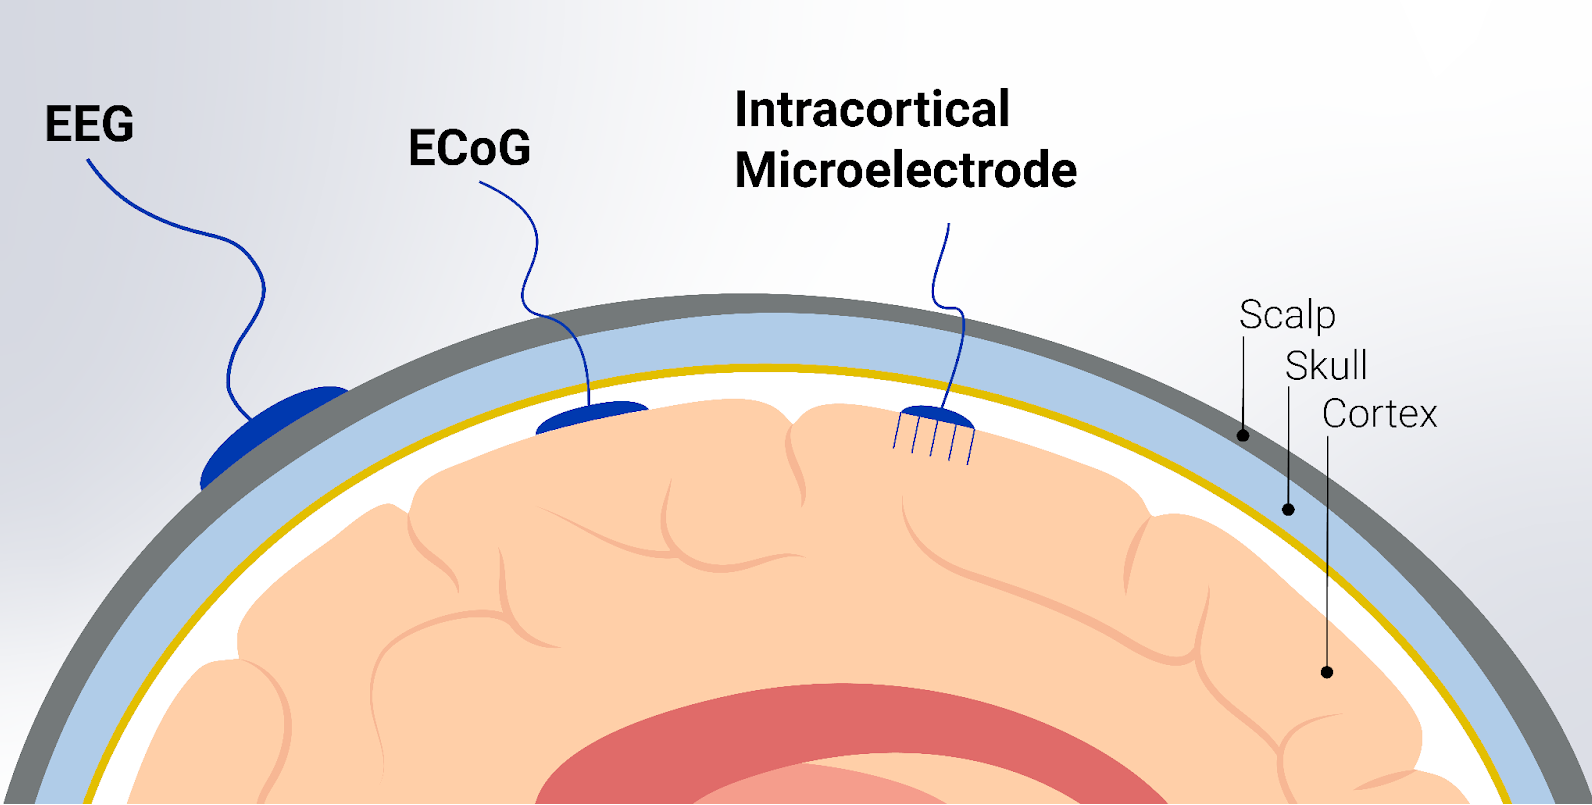
\includegraphics[scale=0.35]{gfx/SuI3_BCI_locations.PNG} 
    \caption{Overview over different recording sites of BCIs \cite{ONLINE:BCI_LOC}}
    \label{def:bciLoc}
\end{figure}

However, despite showing optimal signal quality for their applications, having these kind of BCIs come with some big disadvantages. The first and most obvious one is that a surgical procedure is required to insert the electrodes under the skull and on top or inside the brain, bringing the complications of surgery and recovery from such a procedure with it \cite{zhao-2023}. 
Furthermore, having any device placed on the brain with a surgical procedure requires greater reliability of the implanted device, which, in turn, not only makes the updates to the hard and software of invasive BCIs more complex but also significantly increases their overall cost \cite{zhao-2023}.

\subsection{Non-Invasive BCI}
\label{sec:def:non-invasive}

Non-invasive BCIs are BCIs that do not require any surgical procedure for collection of the required brain signals, which also presents as their most important advantage over the invasive BCI. Typically, the electrodes for measuring the brain activity are placed on top of the head where, in the case of using so called \emph{wet electrodes}, they are connected to the human scalp using a conductive gel to ensure stable electrical transmission.
\emph{Dry electrodes}, on the other hand, do not use any form of conductive gel and are instead placed directly on the scalp \cite{usakli2010improvement, yadav-2020}. 
To hold the electrodes in position for recording and to ensure they remain connected to the head during possible movement, they are usually placed on a so-called electrode caps, which feature preset openings for the electrodes to fit in (see Fig. \ref{def:bciNonInv}) \cite{usakli2010improvement}.

\begin{figure}[h]
    \hspace*{-0.0cm}
    \centering
    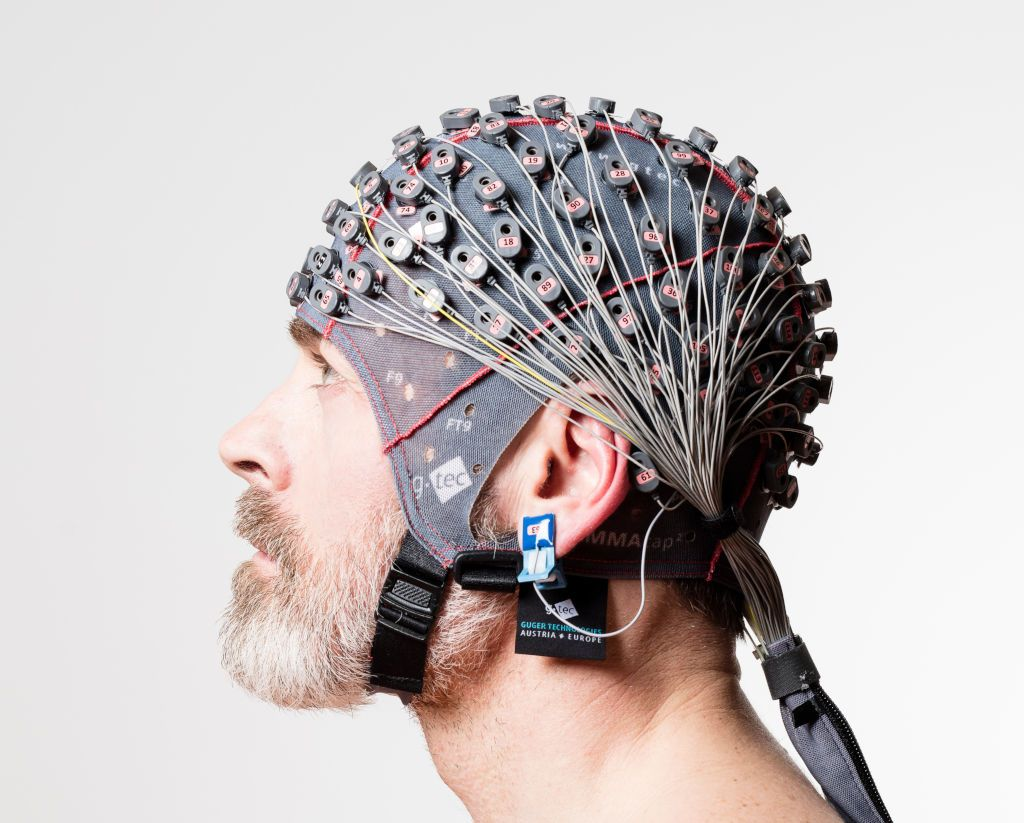
\includegraphics[scale=0.3]{gfx/SuI3_non_invasive_bci_gtec.jpg} 
    \caption{Example for electrode placement in non-invasive BCIs \cite{ONLINE:BCI_NIV}}
    \label{def:bciNonInv}
\end{figure}

While not needing surgery to be used, the recorded brain signals from non-invasive BCIs mainly suffer from lowered signal resolution and error sources (so-called \emph{artefacts}) such as movement, eye and noise artefacts \cite{waldert-2016}.
Other disadvantages and challenges of non-invasive BCI, including those specific to their use in gaming applications are discussed later in this paper in Chap. \ref{chap:challenges}.


\section{Frequency bands}
\label{sec:def:freqBand}

Brain signals tend to vary in frequency depending on what mental state the mind finds itself. The frequencies are summarised into so-called ``frequency bands'', which are listed and briefly explained in the following list, based on the one provided by Yadav et al. in their recent review of BCIs \cite{yadav-2020}:

% maybe turn into table?
\begin{itemize}
    \item \textbf{Delta} (\emph{1 - 3 Hz}): Normally only occur during deep sleep
    \item \textbf{Theta} (\emph{4 - 7 Hz}): Occur during sleep, drowsy or meditation states
    \item \textbf{Alpha} (\emph{7 - 12 Hz}): Occur while the brain is in a relaxed state
    \item \textbf{Beta} (\emph{12 - 30 Hz}): Occur during active thinking, concentration and alertness
    \item \textbf{Gamma} ( > 30 Hz): Occur while brain is processing and recognising external stimuli such as touch or sound
\end{itemize}

\section{BCI paradigms}
\label{sec:def:paradigm}

There are several established ways to acquire brain signals to be able to operate BCIs, summarised under the term of ``BCI paradigms''. These BCI paradigms can be differentiated according to whether they require an external stimulus (event-related potentials) for  operation or work without needing one (spontaneous potentials). 

\subsection{P300 signals}

A special % and widely used? can we back that up?
kind of Event-Related Potential (ERP) come in the form of the so-called ``P300 evoked potentials''. These potentials occur in reaction to a rarely occurring stimulus among an array of regular and systematic stimuli, termed ``oddball stimulus''. % cite
Such a potential can be triggered by asking a user to concentrate on a letter of their choice in a given matrix of letters on a computer screen (see Fig. \ref{def:P300}) while the computer randomly flashes through all of the available entries of the matrix individually. Approximately 300 ms after the chosen letter of the user is then randomly flashed, a potential can be registered in the brain activity of the user and thus said flashed letter can be correctly attributed to the letter the user chose to think about and concentrate on. Furthermore, it has been reported that the less likely the stimulus is, the higher the amplitude of the signal elicited by the oddball stimulus is. %cite!
% add sth about that it's not really usable for our cases? could then say that it might pose an accurate way to maybe move a character in an environment but is faaaar to slow for real use

\begin{figure}[H]
    \hspace*{-1.0cm}
    \centering
    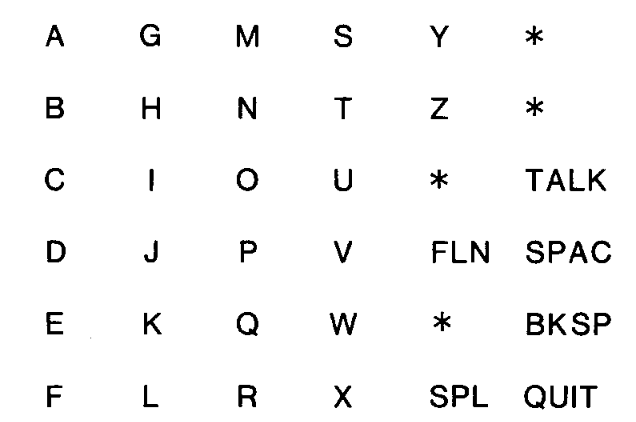
\includegraphics[scale=0.5]{gfx/MThes_P300Matrix.png} 
    \caption{Example of a P300 letter matrix used to mentally type out words for the computer to  voice out \cite{farwell-1988}}
    \label{def:P300}
\end{figure}



\subsection{Steady-State Visually Evoked Potentials (SSVEPs)}

Steady-State Visually Evoked Potentials (SSVEPs) are a particular kind of Evoked Potentials (EPs), which themselves are a subset of ERPs. EPs are potentials which can be recorded when the brain is focusing attention on an external stimulus, like a visual or auditory stimulus and show different characteristics based on the used stimulus \cite{martisius-2016}. 

Visual EPs, which are used in SSVEPs, feature a certain characteristic that makes them highly useful for controlling BCIs: When presented with a visual stimulus in the form of a flickering light source, the potential which is evoked shows the exact same frequency as the flickering light source (See Fig. \ref{def:VEP}) \cite{martisius-2016}.

\begin{figure}[H]
    \hspace*{-1.0cm}
    \centering
    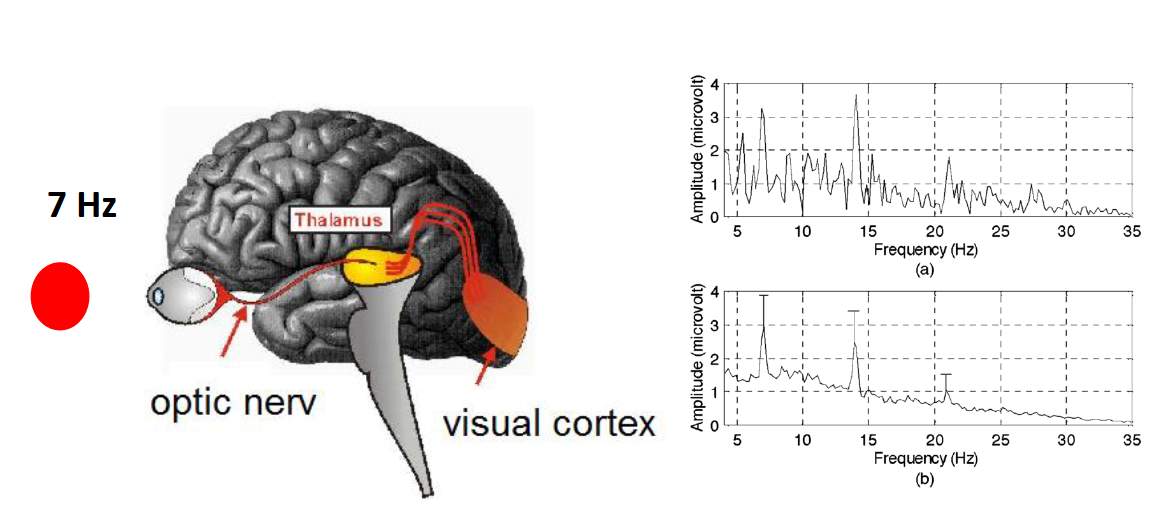
\includegraphics[scale=0.5]{gfx/SuI3_VEP.PNG} 
    \caption{Effects of a flickering light source on the resulting VEP frequency (based on \cite{IMG:VEP})}
    \label{def:VEP}
\end{figure}

SSVEPs use this effect to show multiple flickering light sources, each flickering at their own distinct frequency, to determine which light source the user is currently focusing their attention on at any given moment. This allows a clear classification of the resulting neural responses, as opposed to the area estimation of the regional brain activity evoked during spontaneous potentials. \cite{martisius-2016}. % rephrase?

\begin{figure}[H]
    \hspace*{-1.0cm}
    \centering
    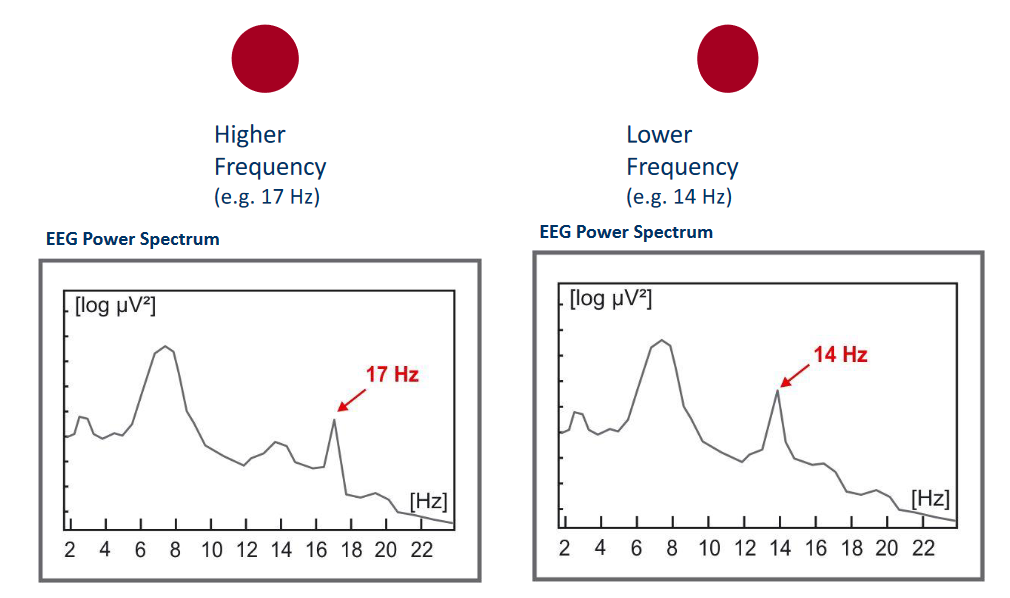
\includegraphics[scale=0.45]{gfx/SuI3_SSVEP_official.PNG} 
    \caption{Example usage of different flickering frequencies for SSVEP (based on \cite{IMG:SSVEP})}
    \label{def:SSVEP}
\end{figure}

\subsection{Spontaneous Potentials}
\label{sec:def:motim}

Spontaneous potentials, as mentioned before, can occur without the need of an external stimulus to be present \cite{martisius-2016}. They are recorded over a time span of a few seconds while brain activity is present in different frequencies (see Section \ref{sec:def:freqBand}) and in different regions of the brain. A combination of both a specific brain region and a specific frequency band can be attributed to a specific mental task (see Image \ref{def:SpontPot}) which then can be used to issue a specific command to the BCI \cite{martisius-2016}. 

\begin{figure}[h]
    \hspace*{-0.7cm}
    \centering
    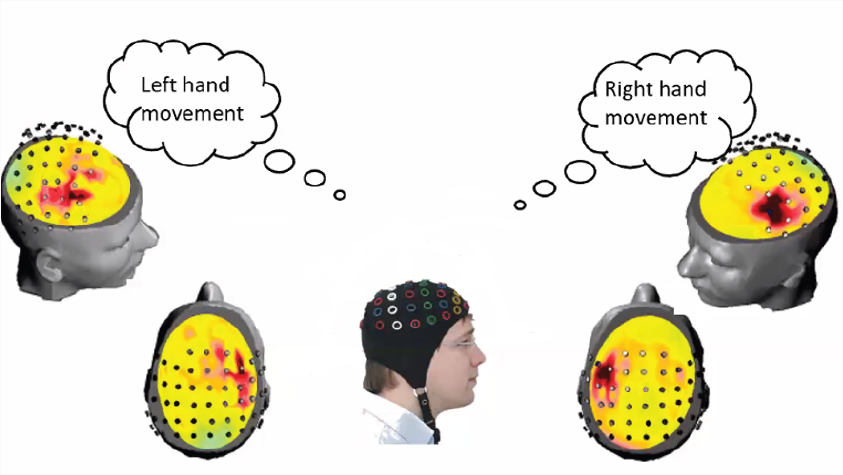
\includegraphics[scale=0.5]{gfx/SuI3_Spontaenous_potential.PNG} 
    \caption{Example of brain activity for specific mental tasks (based on \cite{IMG:SpontPot})}
    \label{def:SpontPot}
\end{figure}

\subsection{Motor Imagery (MI)}

Motor Imagery (MI) is a specific BCI paradigm in the category of spontaneous potentials, which uses the mental imagination of a movement without physically executing it. During MI, brain activity can be recorded in similar regions of the brain as during actual execution the movement, especially in areas of the sensorimotor cortex, where movement is planned and processed. % cite, is that clear and helpful for understanding?
These changes are commonly observed in the mu (8–13 Hz) and beta (13–30 Hz) frequency bands (see for reference Sec. \ref{sec:def:freqBand}) and are characterised by event-related desynchronisation (ERD) and event-related synchronisation (ERS), where the a change in power of specific frequency bands can be recorded, depending on the performed imagined movement task. % phrasing ok?

% might also take the picure from before in here and use a different one to symbolise spontaneous potentials (might be more clear)

In BCI applications, these signal changes can be detected and classified in order to translate imagined movements, such as imagining movement of the left or right hand, into control commands for external systems, like a game controller. % fitting?


% I think it's best to briefly describe the diferent paradigms here, especially P300, keep SSVEP and end with MI, where we just extend our already written section
% keep alphawow + butterfly game, omit neurosky, keep elden ring
\section{Neural Network architectures and algorithms}

Neural Networks (NNs) have been found to be useful in the use of classifying EEG data for their use for BCIs. % cite 
To get an understanding for the different types of NN used with BCI, especially in the examples presented in Chap. \ref{chap:relWork}, this section introduces the most common forms of NNs that can be used in BCI applications. % phrasing ok?

\subsection{Convolutional Neural Networks (CNNs)}

Convolutional Neural Networks (CNNs) are a type of NN that, while functioning similarly to classical NNs, are primarily
used for image processing \cite{oshea-2015}. % ciiiite
A distinctive feature of CNNs is that they can compute an output for an entire image region
using so-called “convolutional layers” (Convolutional rather than from each individual pixel, thereby significantly
reducing the number of parameters to be calculated \cite{oshea-2015}. % ciiiiiite (take the ones from our bachelor thesis)
% plus add a section how they can be used for our EEG data (extracting spatial and temporal features n stuff :3333, would fill this section + provide a bit of clarity about the terms so we don't have to specifically do a section for them cc:)


\subsection{Transformer}

% vvvvvvvvvvvv Translated stuff from our previous thesis: rephrase!
Transformers are based on the principle of \glqq attention\grqq, which enables the network to identify highly relevant parts of the input data and then highlight them. % cite!
In the case of translation, where the input sequential data consists of the words in the input sentence, attention would be helpful here to highlight words relevant to the context for the translation.

In the landmark paper \glqq Attention is all you need\grqq \space from 2017 \cite{vaswani-2017}, the Transformer was introduced as a model for sequence translation. This model, which, as was customary at the time, consisted of an encoder and a decoder connected by attention mechanisms, did, however, completely dispense with recurrences and convolutions for the first time.

Instead, the entire network architecture was based on attention mechanisms, thereby surpassing the performance of the previously best architectures for translation tasks.

Although a Transformer consists of both an encoder and a decoder, only the encoder of a Transformer will be examined in detail below, as it is the only component used in the architecture of the novel network architecture \acl{ViT}.

According to the paper, a Transformer's encoder consists of six stacked encoder layers, each composed of identical sublayers.

In the first sublayer, the input data is processed by a so-called ``multi-head self-attention” mechanism. Multi-head attention
is a concept for attention mechanisms in which the input data, instead of passing through a single attention layer, is processed in parallel through multiple attention layer and the results are subsequently combined and linearly mapped. Self-attention, in turn, is a mechanism that allows the remaining elements of the same sequence to be considered in the case of sequential data, thereby enabling contexts within the sequence to be identified and highlighted accordingly. The second part of the sublayer consists of a fully connected ``feed-forward network” that feeds the sequential input data from the ``multi-head self-attention” layer, regardless of their order, into the next, identically structured, encoder layer. At the end of each sublayer, the output data is normalized and added to the input data of the respective sublayer. % check + cite the correct paper!

% + add relevant picture if neeeded :3 (just have to see that it's not toooooooooo cmplex, as we only use transformer briefly in rel works and maybe as a possible approach, you got this :3)

% also add stuff about the decorder! (prob from the same paper)

% ^^^^^^^^^^^^^ reeeeeephraaaase :33333

\subsection{Common Spatial Patterns (CSP)}

Common Spatial Patterns (CSPs) is a spatial filtering method that is used in signal processing and is especially helpful in BCIs for extracting features from brain signals across multiple EEG channels. % cite? :,3
It was originally introduced by Koles et al. in their paper ``Spatial patterns underlying population differences in the background EEG” in 1990, where this method was proposed for analysing differences in EEG activity between different human populations \cite{koles-1990}.
Later, the approach was popularised and adapted for BCI applications by Ramoser et al. in the year 2000 by using subject-specific spatial filters for discriminating between left- and right-hand movement \cite{ramoser-2000}.% ciiiiite

\begin{figure}[h]
    \hspace*{-0.7cm}
    \centering
    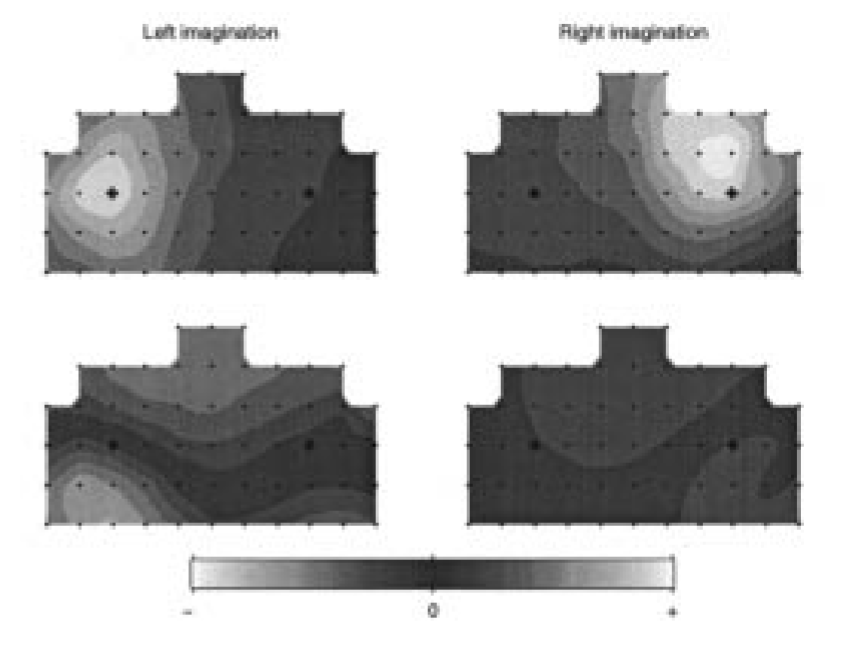
\includegraphics[scale=0.8]{gfx/MThes_CSPPatternVis.png} 
    \caption{Visualization of determined spatial filters for imagined left and right motor imagery across the EEG electrodes with lighter shading indicating high variance in that specific area (taken from \cite{ramoser-2000})} % is the description correct? should be well summarised
    \label{def:CSPVis}
\end{figure}

The method aims to find such filters which maximise the variance for one class of signals, like imagined left-hand movement while simultaneously minimising it for another class, like right-hand movement, thus aiding in increasing the separability between different MI tasks. Mathematically, this is achieved by computing covariance matrices for two signal classes and solving a generalised eigenvalue problem, % do we know what that is? :p
resulting in spatial filters that project the EEG signals into components with maximal discriminative variance differences (see for reference Img. \ref{def:CSPVis}) \cite{koles-1990}. % rephrase 'cause this is still heavily ChatGPT (or do we? It's really well written :,3) might just focuse on rewriting the last part of the sentence wiuth components n stuff
The extracted features can then be used as input for classification algorithms such as the ones presented in Chap. \ref{chap:relWork}.

% CSP are first and foremost a signal processing technique! (so not a 'real' pattern, sadly :,3)
% -> AI summary: Common Spatial Patterns (CSP) a supervised signal processing technique used to design spatial filters that maximize the variance (power) of electroencephalogram (EEG) signals for one motor imagery task while minimizing it for another. 


\section{Applications of BCI in gaming}
\label{chap:applications}


The following paragraphs present existing applications of BCIs in gaming, while also trying to showcase the usage of different BCI paradigms (see Chap. \ref{sec:def:paradigm}) used for controlling them. % might adapt and rephrase



\subsection{AlphaWoW by Nijholt et al.}

In 2009, Nijholt et al. published an article discussing the potential of using BCIs in gaming applications, giving examples for different already existing applications but also showing an application using BCI they developed themselves, which they called ``AlphaWoW'' \cite{nijholt-2009}. \emph{AlphaWoW} (see Fig. \ref{app:alphaWoW}), which is short for ``Alpha World of Warcraft'' is a BCI implementation developed for the Massive Multiplayer Role Playing Game \emph{World of Warcraft}, in which the player plays a character in a vast fantasy world, inhabited by other players' characters and characters controlled by the game system \cite{nijholt-2009}.

In this game, players can choose among different variations of characters to play which change their appearance and their abilities they can use to progress in the game. For the experiment, a Night-Elf Druid was chosen as the character to play the game, who has the ability to shape-shift themselves into a bear and back. Using a BCI, Nijholt et al. then made the transformation dependent on the users alpha brain wave activity (for reference see Chap. \ref{sec:def:freqBand}). While the player was relaxed and thus a high activity in the alpha range was being recorded, the player would remain in its Night-Elf Druid form. Once the BCI detected low activity in the alpha range, meaning that the player was less relaxed, more alert and experiencing stress, the BCI made the character shape-shift into its bear form \cite{nijholt-2009}.


\begin{figure}[h]
    \hspace*{+0.3cm}
    \centering
    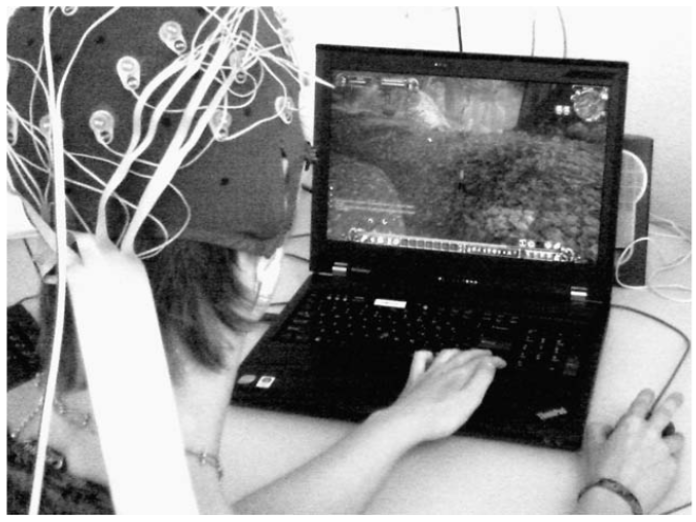
\includegraphics[scale=0.5]{gfx/SuI3_AlphaWoW.PNG} 
    \caption{User playing World of Warcraft using mouse, keyboard and the BCI developed by Nijholt et al. \cite{nijholt-2009}} % rephrase?
    \label{app:alphaWoW}
\end{figure}

Both forms had their advantages for managing enemies in the game. In bear form, the player had increased durability while also dealing high close range combat damage and in Night-Elf druid form, the player could manage dealing with enemies form afar with ranged spells but also had significantly less durability. Most importantly, only while in Night-Elf Druid form, the player was able to heal themselves should they have taken damage in combat with enemies. Thus, the player had to learn to use the BCI to their advantage, relaxing themselves when they wanted to heal themselves and battling enemies form afar and stressing themselves if they wanted to switch to the Night-Elf Druid's bear form for strategical reasons. Using this application, Nijholt et al. noted, the users got satisfaction out of the challenge of having to incorporating this system into their gameplay, showing a possible use of different brain wave ranges for controlling specific action inside a game \cite{nijholt-2009}.

\subsection{Character Controller using SSVEPs through in-game objects}
\label{sec:app:butterfly}

In the context of a game, just having flashing lights at different frequencies to record SSVEPs for a BCI might be off-putting, potentially decreasing the immersion into it. A possible solution to integrate SSVEP triggers into a game in a more natural way was shown in a paper by Legény et al. in 2011 where they presented an SSVEP-based BCI which allowed the user to control their movement in a Virtual Reality (VR) environment in their own pace \cite{legeny-2011}.

For general navigation, three butterflies were constantly shown on the screen, flapping their wings at different frequencies and each corresponding to a direction of movement throughout the virtual space (see Fig. \ref{app:butterflies}). Additionally, to give the user real-time feedback on whether their concentration on a butterfly was successful or not, the BCI would make the antennas of a specific butterfly cross, if it detected focus on that exact butterfly and make the antennas go further apart when sensing that the user was not concentrating on that specific butterfly.
Therefore, to move through the virtual space, the user first had to focus on a butterfly representing the movement direction of their choice and then keep concentrating on it. As long as the BCI recorded concentration on that specific butterfly, it would continuously move the user in that direction until the concentration was either lost or the BCI recorded that another butterfly was being focused on.

\begin{figure}[h]
    \hspace*{-1.0cm}
    \centering
    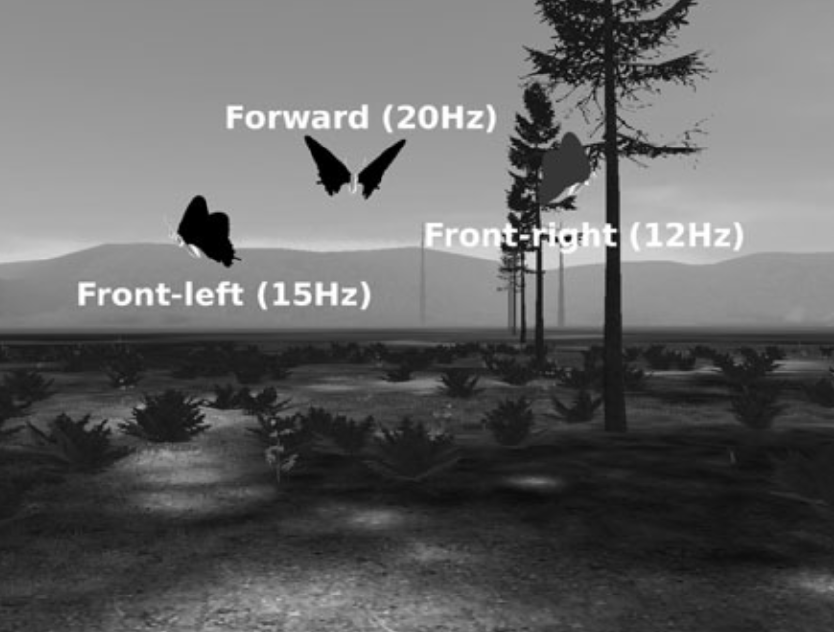
\includegraphics[scale=0.5]{gfx/SuI3_SSVEP_butterflies.PNG} 
    \caption{Butterflies flapping wings at different frequencies for character control in a virtual space using SSVEPs \cite{legeny-2011}}
    \label{app:butterflies}
\end{figure}

The BCI was then tested in an experiment, which aimed to analyse movement performance against movement with keyboard and mouse as well as analysing subjective criteria of the participants, like the feeling of presence in the given virtual world, using both the character controller (i.e. the butterflies flapping their wings) and its real-time feedback (i.e. the crossing antennas). In the same experiment, the butterfly overlay was also compared to a classic SSVEP overlay with flickering lights.
The participants were first asked to complete a training session, where they learned to use the BCI and calibrated the classifier of the BCI which was identifying in what direction the users wanted to move. After training, they were asked to move their character, which was shown in a VR world set in a virtual forest, around five trees to cross a finish line at the end. Additionally, they were given a time limit of eight minutes to complete the slalom trial.

Aside from the expected observation that movement using keyboard and mouse was significantly faster than movement using the BCI, results showed that more than half of the participants were able to complete the trial inside the given time limit of eight minutes. Moreover, results showed that, during the trial, participants were feeling more present in the virtual space using the butterflies for their movement control as opposed to moving through the virtual forest using a classic SSVEP overlay with flickering lights.

\subsection{Emulating a controller using BCIs}

A rather recent example for using a hybrid BCI controller for gaming is presented by the ``video-game and variety streaming-video broadcaster'' \cite{nolan-2023} Perri Karyal \cite{nolan-2023}.
Karyal developed a hybrid BCI controller using a 14-channel headset (see Fig. \ref{chall:emotiv}) for playing the game \emph{Elden Ring}, released in 2022, in which a character moves through an open world and defeats enemies to reach the end of the game's story. Using this headset she was able to issue mental commands that would be translated into attack (see Fig. \ref{out:perri}), spell casting or dodge actions inside the game by having certain mental visualisations of the commands, thus evoking  spontaneous potentials in the brain (for reference, see Chap. \ref{sec:def:spont}). 

\begin{figure}[h]
    \hspace*{-0.2cm}
    \centering
    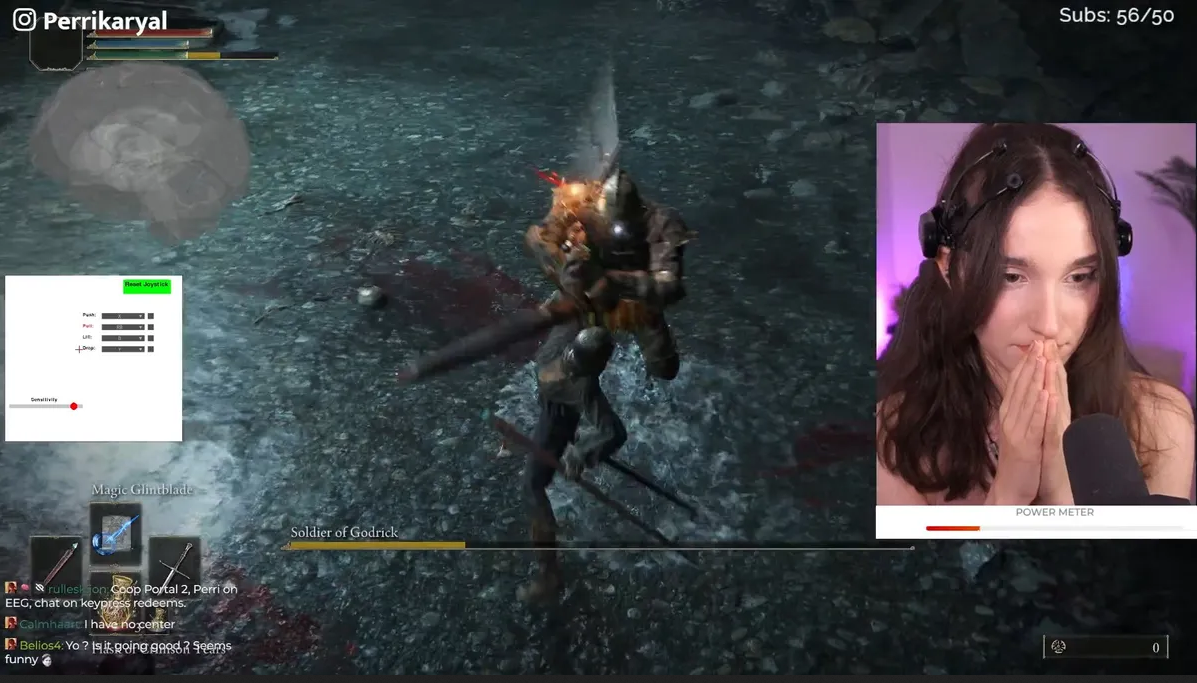
\includegraphics[scale=0.45]{gfx/SuI3_perri_karyal.PNG} 
    \caption{Stream screenshot showing Karyal playing \emph{Elden Ring} where the attack command has just been detected by her BCI (taken from \cite{nolan-2023})} % rephrase?
    \label{out:perri}
\end{figure}


As an example, in order to issue the attacking command inside the game, Karyal would visually imagine ``pushing something forward in [her] head'' \cite{nolan-2023}, which would increase brain activity in a specific region of the brain which could then be detected by the BCI to issue that specific command. By using additional head-tracking for movement she was later able to create a full hands-free controller for that game \cite{nolan-2023}.
While this recent development looks promising for future applications of BCIs in modern games, Karyal herself stated, that in order for the BCI to recognise the commands as accurately as possible (and as shown in her videos), she had to spend more than 250 hours just for calibrating the headset to her mental visualisations \cite{nolan-2023}, bringing us back to the issue of training, one of the main challenges of using BCIs in gaming applications (see Chap. \ref{chall:training} for details).

\section{Relevant challenges}
\label{chap:challenges}


% might also have to restructure this chapter to be more understnading and in line with our actuial thesis goal

The usage of BCIs in gaming applications, however, comes with its own extensive set of challenges. In this paragraph, they are summarised under the most important aspects, while trying to give both concrete examples for their issues in gaming applications and also proposing possible solutions for them, where possible.

% mention that BCI, for now, probably will never be able to be used in fast-pced settings like action games (actually  might put that into conclusions! could be interesting)

\subsection{Signal Quality} % section relevant?

The first challenge for using BCI headsets in gaming applications can be found in the quality of the signal recorded from the brain activity itself. As mentioned in Chap. \ref{sec:def:invasive}, an electrode placed directly inside the brain would ensure optimal signal acquisition, yet this approach is definitely not suitable for making BCI games for a large number of users in a non-clinical setting.
Therefore, the examples for BCIs presented in Chap. \ref{chap:applications} are exclusively non-invasive, coming with the advantage of not requiring surgery for their use while accepting the loss in signal quality which comes with it. 
Signal quality is also affected by the number of electrodes used for its acquisition. Generally, the more electrodes (also called ``channels'') are placed on the head (going up to 256 channels \cite{seeck-2017}), the higher the resolution of the recorded signal can be. According to the International Federation of Clinical Neurophysiology (IFCN), the standard amount of channels for recording brain signals in clinical settings was once 32 channels in 1998 but was then updated to 25 channels in 2017 \cite{nuwer-1998, seeck-2017}. % rephrase to reduce mental load reading this? might omit the 256 electrode part or just say hey the standard is 25 deal with ii
BCIs in non-clinical settings use considerably fewer channels, like the SSVEP controller presented in Chap. \ref{sec:app:butterfly}, which uses six channels and thus decreases the overall quality of the signals that can be recorded by them.
A reason for that reduction is that the more channels are present, the more time is required to set up the BCI for the user, especially using wet electrodes (see Chap. \ref{def:bciNonInv} for details), and the more the BCI itself costs. To compromise that, BCIs sold commercially use fewer channels and dry electrodes (see Fig. \ref{chall:emotiv}), reducing setup time but potentially also decreasing their signal quality compared to BCIs in clinical settings.

\begin{figure}[h]
    \hspace*{-0.0cm}
    \centering
    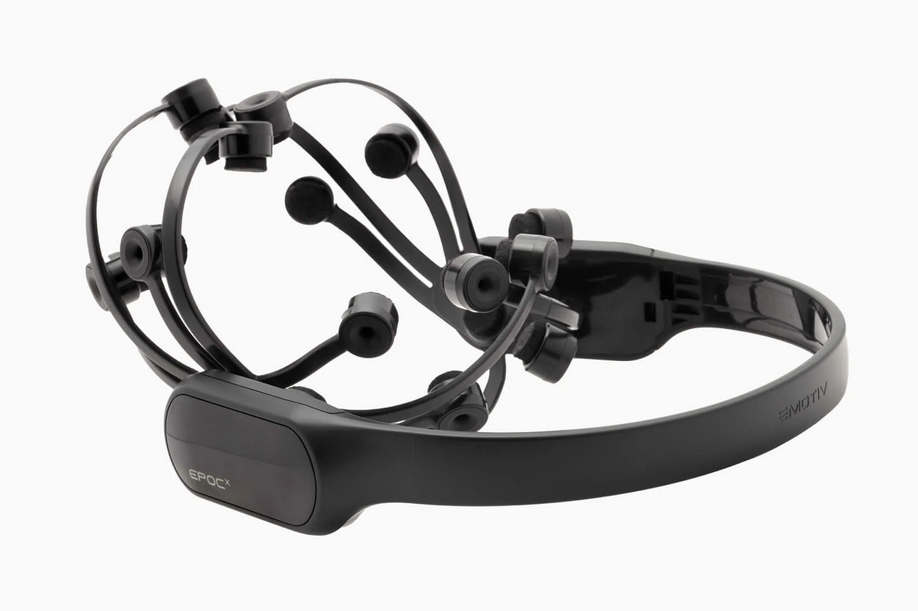
\includegraphics[scale=0.3]{gfx/SuI3_emotif_epoc.PNG} 
    \caption{A 14-channel headset for brain signal acquisition sold by \emph{EMOTIV} (taken from \cite{EMOTIV:EpocX})}
    \label{chall:emotiv}
\end{figure}

[Go into more detail here!] % might also mention the issues in otur actual implementation chapter and note how we solved the issues and which algrotihms we used in order to do so
Additionally, signal quality in non-invasive BCIs is further decreased with error sources such as head, eye and muscle movement of the user (mentioned in Chap. \ref{sec:def:non-invasive}). To reduce that kind of loss in signal quality and to increase the reliability of BCI to correctly translate brain signals into potential control commands, the incoming signals can be filtered using a range of different methods including those frequently used in machine learning % can go into a bit more detail here, since we do write our master thesis
\cite{abdulkader-2015}.


\subsection{Transfer Rate}

% insert the image about transfer rate here (if it still exists and we find it)

Another issue in using BCIs in gaming applications is their low transfer rates of issued mental commands to evoke action on the screen, especially compared to the transfer rate of a keyboard and mouse. 
For BCIs, the transfer rate can be derived from the Information Transfer Rate (ITR), which is used as a metric to assess a combination of the BCIs selection time, number of choices and recognition accuracy \cite{yadav-2020}. For evoked potentials that use an external stimulus, like the SSVEP, the ITR ranges between 60 and 100 bits per minute \cite{yadav-2020} meaning that one bit of information can be transferred approximately every 0.75 seconds, whereas keyboards take around 0.05 to 0.1 seconds to transfer information about a key press \cite{casiez-2017, wimmer-2019}. The time difference in using SSVEPs compared to a keyboard was further shown in the SSVEP controller by Legény et al. (shown in Chap. \ref{sec:app:butterfly}), where the authors reported, that the users were able to complete the virtual slalom course four to seven times faster on keyboard then they did using the SSVEP controller \cite{legeny-2011}.

This could pose a problem for the application of BCIs in fast-paced games like shooters or others action games. A possible solution for that might be either choosing to develop BCI games with less time-critical game elements or using a hybrid input system which uses both BCI input and traditional input like keyboard and mouse or touch, as seen in \emph{AlphaWoW} and specifically Karyals BCI controller for \emph{Elden Ring}, which serves as a defining inspiration for the BCI controller used in this thesis for the evaluation of our different calibration algorithms.

\subsection{Training}
\label{chall:training}

The last major and, in the context of using BCIs in gaming applications, most pressing issue is the significantly high time needed to train BCIs. 
In order for the BCI to correctly and rapidly translate the brain signal inputs of a user to a corresponding action, the BCI has to be extensively calibrated to the inputs of the user. Additionally, the user also has to spend some time to figure out how to support the BCI in the classification of their signals, for example by focusing on being relaxed to make it easier for the system to detect activity in alpha range or choosing mental commands % defintiely reference mental commands in spontaneous potentials too and refere to the EMOTIV site for mental commands (as long as they somehow are backed by science, could always say, that they are called mental commands by some companies and insitutions producing/manufacturing BCI)
that are easier detected by the BCI. Thus, in a way, both the BCI and its user have to undergo some form of calibration to learn to ``understand'' each other in order for the BCI to function properly and accurately \cite{nijholt-2009}.

Generally speaking, the more time is spent training the BCI and its user, the more precise the results can be \cite{nijholt-2009}. 
However, in gaming applications, this extended training time might be bothersome to perform before even playing the game, resulting in a barrier for playing games that use BCIs for controlling it. For that reason, Nijholt et al., in their paper ``Turning Shortcomings into Challenges: Brain-Computer Interfaces for Games'', suggested integrating BCI calibration directly into the game (e.g. by using an in-game tutorial before the actual game) \cite{nijholt-2009}. Nijholt et al. also mention, that this definitely asks game designers to incorporate adequate levels and game elements requiring BCI control to be solved successfully into their games to enable such form of integrated calibration \cite{nijholt-2009}. 
This represents the main underlying issue of using BCIs in video games which the algorithms presented and used in this thesis aim to minimise and contain. % prob def rephrase xd
% might close the challenges subsection with a transition to 

[also mention inter-session + inter-subject variability here!]
[-----------]

[Now follows the intro to the technical stuff like the specific algorithms, Neural Networks, CNN,etc!]

Current stuff:

CNN?
Transformer % yes! Will have to explain both CNN and Transformer briefly


[----------]

(but also stuff like temporal resolution and all the stuff that might be new in the related work so people understand what we're actually talking about CC:)

% also might have to restructure afterwards if needed uwu

% might actually also use stuff from our bachelorthesis if we talk about different networks like CNN n stuff

% vvv will be needed once we definitely know which kind of algorthims we will use, so it's wise to just wait for thesis progression in order to exactly know what needs to be defined still
% might need to think about defining algorithm stuff too, depending on what they entail, might also ask Guthe about it if we should also introduce the readers to neural nets or if that's a given once you are in this field already (might actually be redundant since we come from comp science), might think about defining specific parts of the algorithm if they go above and beyonf the 'classic' neural network stuff                                                                                                                                                                                                                                                                                                                                                                                                                                                                                                                                                                                                                                                                                                                                                                                                                                                                                                                                                                                                        
\chapter{Related Work}
\label{chap:relWork}

This chapter will show the different approaches found while researching related work for the reduction of calibration time for BCIs. %rephrase?
While most of the papers % if not all
are not specifically using BCIs as part of an input device for a video game, the saved time during calibration is an important factor no matter the concrete application of the BCI.

% do we need a more recent paper? :,,,,,33 (might ask guthe about that)
\section{Using Transfer Learning with previously recorded sessions}
\label{sec:relWork:TL}

In their paper ``Reducing Calibration Time For Brain-Computer Interfaces: A Clustering Approach'', released in 2006, researchers Klauredat et al. analysed an approach how to reduce mentioned calibration time of BCI by using data from previously recorded sessions of BCI users \cite{krauledat-2007}. 
As the main underlying problem of the calibration overhead, the authors mentioned the difference in data across multiple sessions due to factors like fatigue of the user and possible different approaches in imagining the mental for the BCI. Thus, in order to reduce the calibration time, they chose to extract the invariant features of each session using machine learning approaches to be able to use them as data for subsequent calibration sessions. For this, they acquired 64-channel EEG data from six individuals, each undergoing at least four sessions using the BCI. The sessions started with a calibration recording phase, during which, approximately every five seconds, the users were asked to visualise one randomly selected motor task out of three motor imaging tasks% possibly use acronym
, namely left and right hand and left for movement. Following the prompt, the system then recorded the users brain activity over a period of around three seconds, afterwards repeating the process between 120 to 200 times per motor imaging task \cite{krauledat-2007}.
The calibration recording phase was then followed by a machine learning phase, in which a classifier was trained to distinguish between the individual motor tasks and then completed by a feedback phase % not closer mentioned in detail by the paper
, presumably to evaluate the classifier by the user.

To extract the common features of the brain data over multiple sessions, the researchers then used three different kinds of Common Spatial Pattern (CSP) algorithm approaches over the underlying recorded brain data of each individual BCI user to detect recurring spatial filters. These three different approaches, shown in Fig. \ref{rel:CSP_Hist} and all eliminating the need for a new calibration session in subsequent sessions, can be summarised as follows:% introduce  CSP in own section in introduction?
\begin{itemize}
    \item \textbf{HIST-CSP}: Using a single set of CSP filters over the collected historical data of previous sessions
    \item \textbf{PROTO-CSP}: Using prototype filters derived from finding recurring clusters of CSP filters among the individual recording sessions
    \item \textbf{CONCAT-CSP}: Concatenating the single set of CSP filters from \textbf{HIST-CSP} with the derived prototypical CSP filters from \textbf{PROTO-CSP}
\end{itemize}

\begin{figure}[H]
    %\hspace*{-1.0cm}
    \centering
    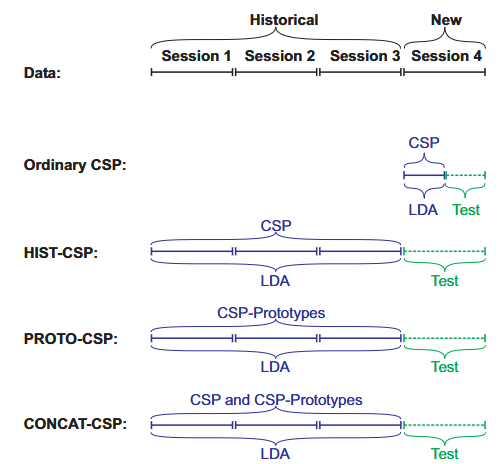
\includegraphics[scale=0.8]{gfx/MThes_CSPHistApproaches.png} 
    \caption{Overview over different CSP algorithm approaches using historical data from previous calibration (taken from \cite{krauledat-2007})}
    \label{rel:CSP_Hist}
\end{figure}

Results (visualized in Fig. \ref{rel:ZeroTrainErr}) show the classification error (in \%) of the individual CSP algorithm approaches used by Krauledat et al. using only historical data for training the classifier and proceeding directly to the feedback phase in new sessions. In contrast, the ordinary CSP approach still uses half of the session for calibration (as seen in Fig. \ref{rel:CSP_Hist}) and the rest of each new session for the feedback phase. The Zero-Training algorithms produced significantly low error percentages in most subjects, especially using the CONCAT-CSP approach, thus proving the feasibility of this approach for the reduction of calibration time of BCI.


\begin{figure}[H]
    %\hspace*{-1.0cm}
    \centering
    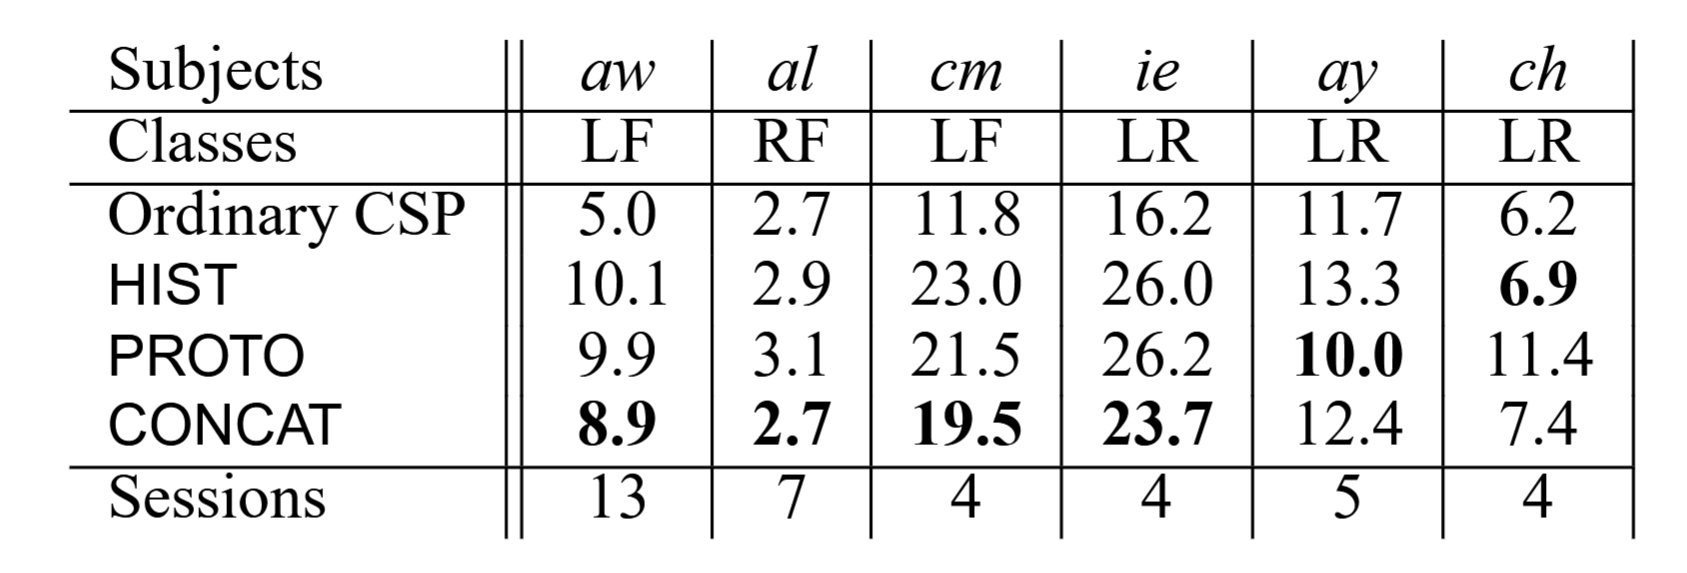
\includegraphics[scale=0.25]{gfx/MThes_ZeroTrainErrorProb.png} 
    \caption{Error rates (in \%) for the Zero-Training mode across the tested subjects with the error rate of the standard CSP as reference (taken from \cite{krauledat-2007})} % update description 
    \label{rel:ZeroTrainErr}
\end{figure}


A more recent study from the year 2022 seems to back up this method, albeit using a different approach in processing and using data of previously recorded data of individual test subjects for new BCI session for the exact same test subjects. % possibly rephrase
In their paper ``A Transfer Learning Algorithm to Reduce Brain-Computer Interface Calibration Time for Long-Term Users'' Giles et al. proposed a method of shortening calibration time for BCI sessions for long-term BCI users down to a few samples taken in each new session \cite{giles-2022}. To use the data from previous sessions, they suggest the use of their proposed r-KLwDSA Algorithm, consisting out of three steps (visualised in Fig. \ref{rel:rKLwDSA}):

% think aboiut if we should use a list or just paragraphs for now
\textbf{1. Data Space Alignment (DSA):} In this step the variance of the data from the previously recorded source sessions was reduced by applying a linear transformation to the recorded EEG data in order to align their data to the new session EEG data \cite{giles-2022} % maybe rephrase?
\newline
\textbf{2. Weighting:} Following that step, the aligned data was then compared to the new session's EEG data and weighted according to the similarities to the previously recorded data, making sure that the variance in data is further reduced by heavily weighing data that is similar to the data from the new session. This data is then used to calculate a covariance matrix of the previously recorded data, the ``transfer learning co-variance matrix'' % do we go more into detail about covariance matrix n stuff? + cite?
\newline
\textbf{3. Fusion:} The aligned data was then fused with the new session's EEG data using a regularization method proposed by Giles et al. which finds the optimal combination of existing and new EEG data by comparing validation accuracies of the individual combinations. Lastly, this data fusion was used to determine the Common Spatial Pattern (CSP) features within it to be able to train the BCI classifier

\begin{figure}[H]
    %\hspace*{-1.0cm}
    \centering
    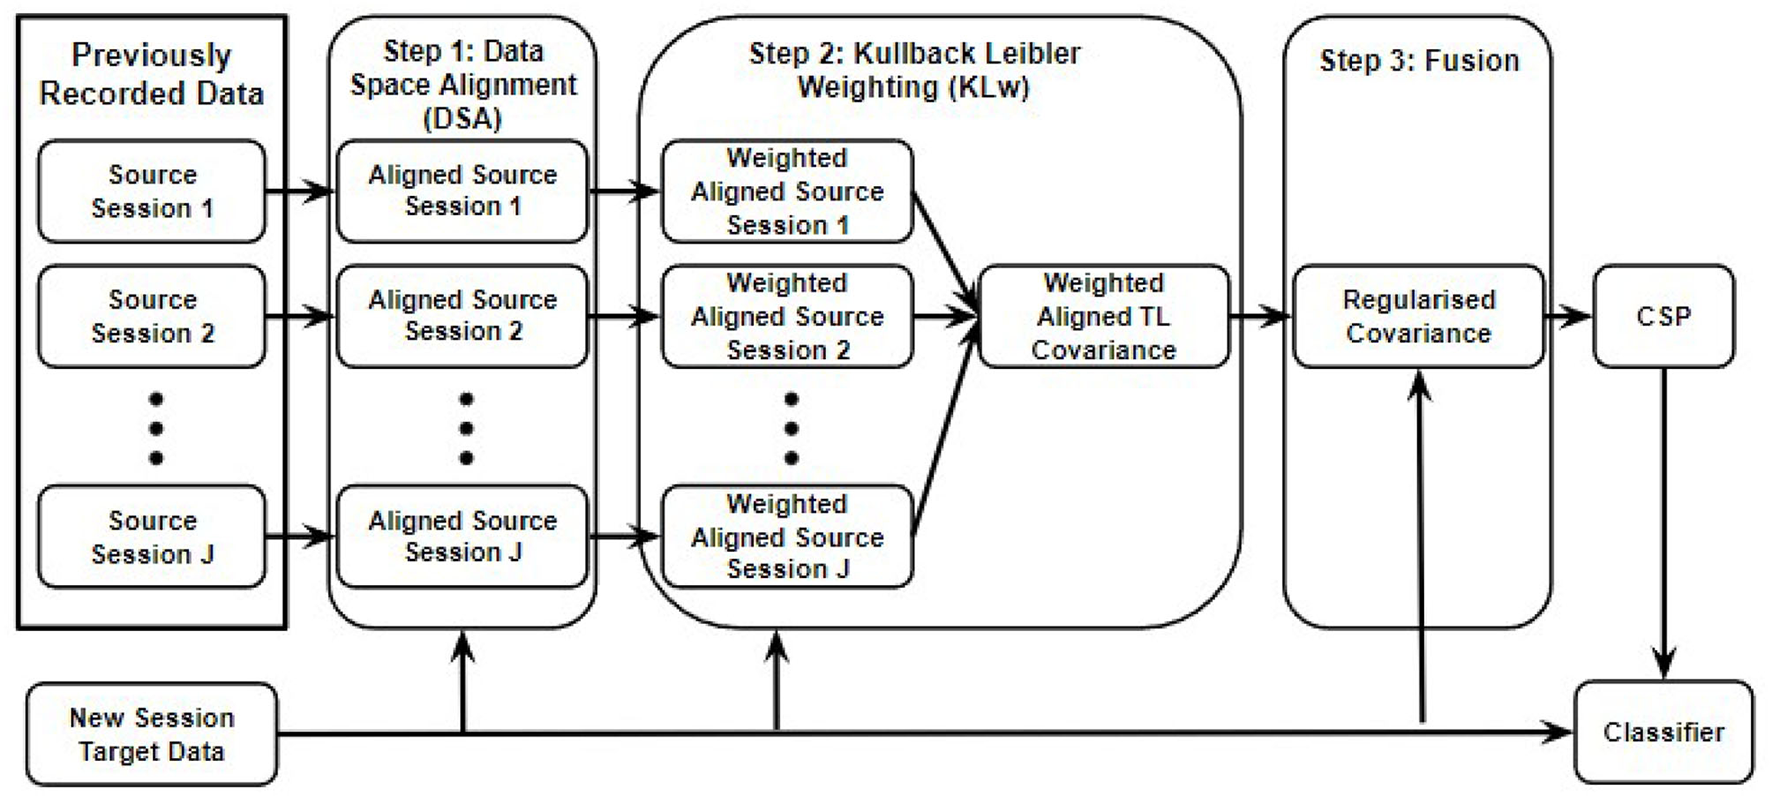
\includegraphics[scale=0.22]{gfx/MThes_rKLwDSA.png} 
    \caption{Overview over the proposed r-KLwDSA algorithm used in the paper of Giles et al. \cite{giles-2022}} % pdate description 
    \label{rel:rKLwDSA}
\end{figure}

Results showed that the proposed r-KLwDSA algorithm outperformed other approaches like using simple DSA or natural Transfer Learning in terms of average classification accuracy \cite{giles-2022}. % prob rephrase

Since, next to the previously mentioned inter-session variability, there is also a high inter-\emph{subject} variability of EEG data across recording sessions, algorithms that account for this variability are desirable for our presented use case. % do we actually mention it? Maybe reference + rephrase

While Kreuledat et al. and Giles et al. used the calibration data of previous BCI sessions of individual test subjects as a basis for removing the need of a calibration session for the exact same test subject, the approaches used in their work can serve as a foundation for an approach using previously recorded data of several different test subjects to shorten calibration time of new test subjects using BCIs, especially since the approaches using data alignment and transfer learning are practically the same for cross-session and cross-subject trasnfer learning \cite{wu-2020}. % rephrase? + mention that the general approach is similar and that the approaches were backed up by the review paper from 2020 by Xu n peeps


- mention CSP filters! (+ try to understand what they actually mean, might help to try to describe CSP in the definitions chapter before c:) [but don't go tooooo far into them, that's not your part in this thesis and doesn't really help our IT(!) (not neuroscience) focused reader group :33, keep it as detailed as needed, BUT! as simple as possible]

% ERD/ERS Event related synchonisation and desynchronsitation (!) Furthermore, it is known since Berger (1930) that certain events can block or desynchronize the ongoing alpha activity.(!) These types of changes are time-locked to the event but not phase-locked, and thus cannot be extracted by a simple linear method, such as averaging, but may be detected by frequency analysis. This means

% From paper:  The filtered signal corresponding to the desynchronization of the left hand motor cortex is characterized by a strong motor rhythm during imagination of right hand movements (left hand is in idle state), and by an attenuated motor rhythm during left hand imagination.
% -> Makes sense, as during thinking of left hand movement the region there is blocked/desynchronised, as it is being used :3

\section{Approaches using Neural Networks}
\label{sec:relWork:NN}

Algorithms, such as the ones presented in the previous chapter, use traditional machine learning and thus rely on an extensive feature extraction process to train a classifier (see for example Img. \ref{rel:rKLwDSA}). % rephrase image ref? + cite?
With the advancements made in the area of deep learning, approaches using Neural Networks can be considered for aiding the sought reduction of the calibration time. For this, according to a review paper on the use of deep learning techniques for classifying EEG Motor Imagery tasks by Altaheri et al. published in 2023, Convolutional Neural Networks (CNN) was the main architecture of Neural Networks used for the implementation of classifiers for said Motor Imaging tasks \cite{altaheri-2021}. Furthermore, the authors also pointed out the ability of the networks to work with raw data with minimal preprocessing to no preprocessing at all \cite{altaheri-2021}, significantly reducing the overhead of the algorithms in comparison to the machine learning approaches from the previous chapter which heavily rely on extensive preprocessing to align the highly variable datasets.% is that clear? Might write about specific papers for reduction of calibration time using CNN now (like 1 to 2 examplpes I guessss)      

An important discovery in this topic was made by Lawhern et al. in 2018, where the authors presented a special type of CNN that is specifically made to be used with EEG signals for Brain Computer Interfaces and is capable to classify EEG data for a multitude of BCI paradigms \cite{lawhern-2018}.% rephrase? 

\begin{figure}[H]
    %\hspace*{-1.0cm}
    \centering
    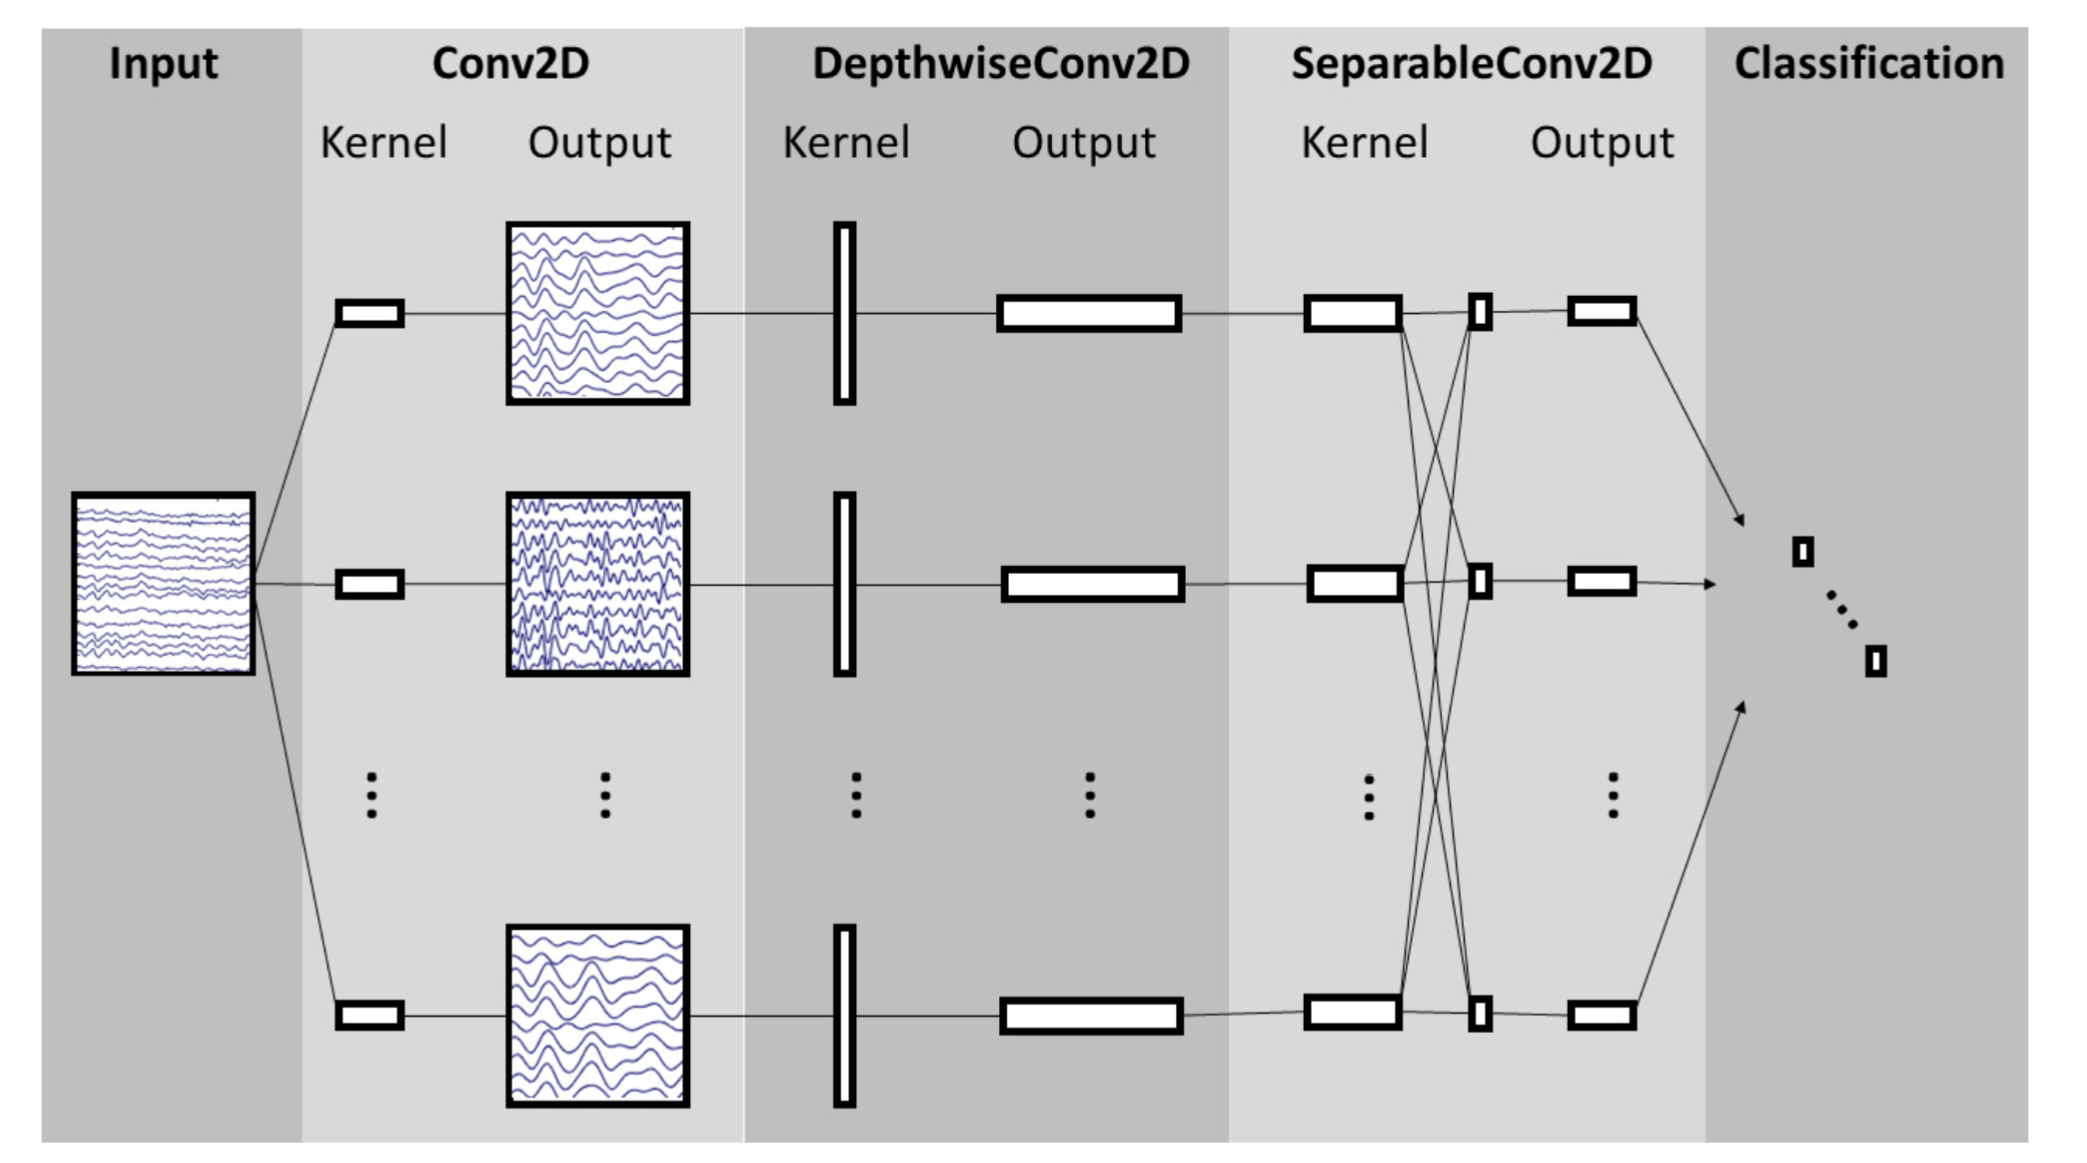
\includegraphics[scale=0.4]{gfx/MThes_EEGNetArchitecture.png} 
    \caption{Visualisation of the EEGNet architecture (taken from \cite{lawhern-2018})} % update description 
    \label{rel:EEGNetArch}
\end{figure}

The architecture of this network (see for reference Img. \ref{rel:EEGNetArch}) handles incoming EEG data as follows: % maybe think about converting this to a list at some point
First, the incoming data is temporally convoluted with a filter size of (1, 64), according to half of the sampling rate used in this paper, to enable the network to extract frequency information for the underlying data. The result of this convolution are feature maps containing EEG data for different frequency bands. % is that correct?
After that, another convolution is applied with a filter size of (n=numberOfChannels, 1) % reformat
which enables the network to extract spatial patterns for specific frequencies \cite{lawhern-2018}.Before the third convolution step, the sampling rate is reduced to 32Hz through an average pooling layer, after which the data is first convoluted with a filter of (1, 16), which represents 500ms of the recorded EEG activity, and then additionally convoluted convoluted pointwise with a (1, 1) filter. According to Lawhern et al. these two separated convolutions in the third convolution enable the network to separately learn to summarize the underlying feature map data in time, corresponding to the depth-wise convolution, and learn how to optimally combine these feature maps, corresponding to the point-wise convolution. Applied to the EEG signal, the authors describe that they first extract a 500ms ``summary'' of each available feature map before combining these summary outputs in the following step \cite{lawhern-2018}. % is that clear? Possibly rephrase (and look at the picture description)                         
% do we put this (from chatgpt) in here too? 
% Overall, the architecture is specifically designed to mimic traditional EEG feature extraction methods such as filter-bank CSP while leveraging the efficiency and flexibility of convolutional neural networks.
A reference of the detailed list of the individual layers used for the EEGNet can be found in the appendix under Img. \ref{app:EEGNetDetail}, which also shows sizes, number of parameters, outputs and possible options depending on layer. % is that clear?

% description from the image of the paper of the architecture: The network starts with a temporal convolution (second column) to learn frequency filters, then uses a depthwise convolution (middle column), connected to each feature map individually, to learn frequency-specific spatial filters. The separable convolution (fourth column) is a combination of a depthwise convolution, which learns a temporal summary for each feature map individually, followed by a pointwise convolution, which learns how to optimally mix the feature maps together. Full details about the network architecture can be found in Table 2

To prove the performance of the EEGNet, the validation accuracy of this network across different BCI paradigms, such as the SMR paradigms which is relevant to our thesis subject, was assessed and compared to other CNN architectures. % are they really all CNN archtiecturres?
A total of two configurations of the EEGNet, ``EEGNet-4,2'' and ``EEGNet-8,2'', were used for testing where the 4 and 8 denote the amount of temporal filters learned during training while the 2 indicates the amount of spatial filters learned per temporal filter \cite{lawhern-2018}.
While the EEGNet showed consistently high validation accuracies for paradigms such as P300 ($>=90\%$)% do we mention the different paradigms in the beginning? of this section? Nmely the four paradigms used in this study
for both inter-subject and cross-subject classification, the EEGNet showed significantly lower validation accuracy for the SMR paradigm for inter-subject and cross-subject classification (see Img. \ref{rel:EEGNetSMRAcc}) compared to other BCI paradigms. % is that clear
Still, the EEGNet consistently matched or outperformed other CNN network architectures in terms of validation accuracy on the individual paradigms and can thus be used as a basis for an approach of lowering calibration time needed for BCI using neural networks. % is that clear? or is that closing this chapter 'too soon?'

\begin{figure}[H]
    %\hspace*{-1.0cm}
    \centering
    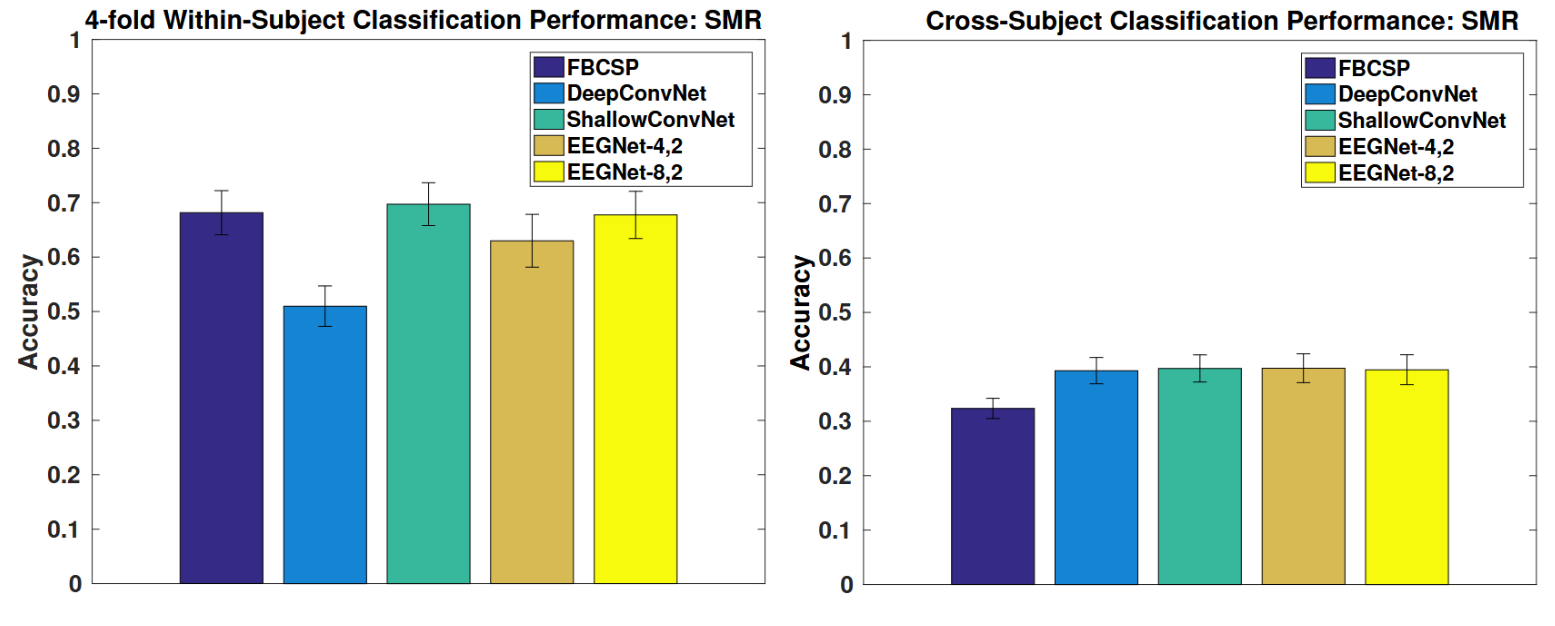
\includegraphics[scale=0.35]{gfx/MThes_EEGNetSMRAcc.png} 
    \caption{Comparison of validation accuracies of the presented EEGNet to other network architectures on both Withing-Subject and Cross-Subject classification (taken from \cite{lawhern-2018})} % update description + explain what 8,2 and 4,2 means c: 
    \label{rel:EEGNetSMRAcc}
\end{figure}

An important strength of the presented network is that it is able to generalize well both while classifying EEG data from the same subject as well as data from different subjects, leveraging the underlying problem of having high inter-session and inter-subject variance of EEG data, which the ML approaches in the previous section tried to address. % rephrase?
Furthermore, the EEGNet proves to be usable for a wide range of BCI paradigms, both ERP, like P300 and SSVEP, and SP like the mental commands performed in task like MI \cite{lawhern-2018}. % rephrase + adjust to recently written results section

Since the publication of this paper in 2018, new and improved architectures of neural networks for classification of EEG data were presented which also show increased validation accuracies for Motor Imaging \cite{salami-2022, wei-2024}. % will we get into detail here? (have tried before but was too complex to go into detail)


% put the detailed layer list into the appendix c:
More recently, in the paper ``Cross-subject EEG Decoding with spatiotemporal transformers for
zero-calibration brain–computer interfaces'' published in 2026, Jiang et al. propose a network based on the architecture of transformers % reference to grundlagen chapter? C:
that is able to accurately classify for Motor Imagery tasks without the need of prior calibration \cite{jiang-2026}, which accurately fits our use case of having a multitude of players use a BCI without prior experience and recorded BCI sessions.  
% chatgpt stuff to maybe add: In contrast to traditional CNN-based approaches, which mainly focus on local spatial–temporal patterns, the transformer architecture is designed to capture long-range dependencies and relationships within EEG signals through self-attention mechanisms \cite{bci-transformer-2026}.

\begin{figure}[H]
    \hspace*{-0.5cm}
    \centering
    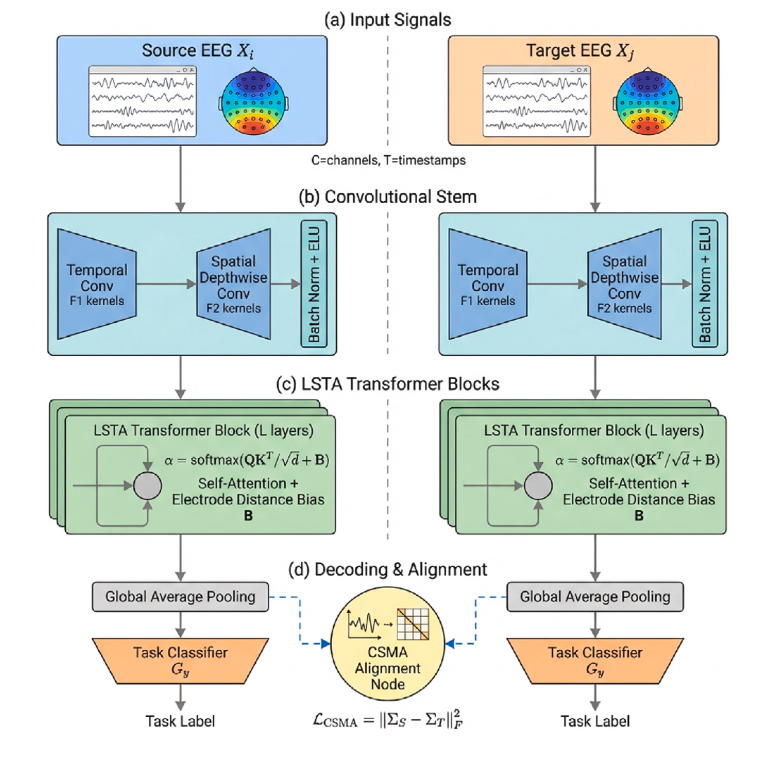
\includegraphics[scale=0.45]{gfx/MThes_BCITransArch.png} 
    \caption{Overview of the BCI-Transformer architecture featuring a dual-stream approach for the source and target EEG data and, LSTA transformer block, and parallel flow through the classifier and the CSMA node (taken from \cite{jiang-2026})} % shorten image description?
    \label{rel:BCITransArch}
\end{figure}

% also mention that it is a hybrid between CNN and tranformer architecture
The hybrid architecture of the proposed network (shown in Img. \ref{rel:BCITransArch}) uses both a classic CNN for spatial and temporal feature extraction and so-called ``Localized Spatiotemporal Attention'' transformer blocks. These blocks focus attention on physiologically relevant electrodes like the electrodes around the motor cortex for MI tasks, compared to classic attention mechanisms in transformers that would attend to all available channels\cite{jiang-2026}. % rephrase?
This initial focus, which can be overridden and is adapted in relation to discovered subject-independent pattern during learning, additionally allows the LSTA blocks to lower subject-specific artifacts in the recorded EEG signals \cite{jiang-2026}.



% now explain the other important step mentioned in the paper :3
Additionally, the network features a Cross-Subject Manifold Alignment (CSMA) node, which aligns the feature spaces of the individual subjects into one shared feature space \cite{jiang-2026}. This reduces distribution shifts and helps the network to learn subject-invariant patterns in the recorded EEG data while still preserving the ability to distinguish between individual classes in the shared feature space \cite{jiang-2026}. % clear? (should be, I think)   
- CSMA (Cross-Subject Manifold Alignment)
% in words of author:  Cross-Subject Manifold Alignment: We define a novel manifold alignment objective (CSMA) that minimizes the discrepancy between the second-order statistics of the latent representations of different subjects, projecting diverse neural distributions into a shared, class-discriminative geometric space.

% in words of chatgpt: The \textbf{Cross-Subject Manifold Alignment (CSMA)} component is used to reduce the variability between different users by projecting EEG data from multiple subjects into a shared latent feature space. Through this alignment process, the model learns subject-invariant representations while preserving class-specific information required for classification. As a result, EEG data from different users becomes more similar in distribution, enabling the classifier to generalise better to unseen subjects without requiring extensive


To prove the performance of the BCI-Transformer, the network was tested on three EEG datasets for Motor Imagery % do we need details? (might ask Guthe)
for zero-calibration capability, representing a possible cross-subject application of the BCI. Results showed that the proposed BCI-Transformer outperformed all 22 networks, across all three datasets, it was compared against achieving validation accuracies 77\% to 88\% depending on the dataset. While the complexity and inference time of the BCI-Transformer was higher than other existing architectures like the EEGNet \cite{jiang-2026}, the achieved validation accuracy of the network in zero-calibration scenarios could outweigh the computational effort needed to use this network architecture. % rephrase?
% append results table into the appendix instead of showing it here?
%  (+ ask pipp how he added an appendix, just to be sure)

This chapter has shown approaches for reducing calibration time through using data recorded from previous sessions (see Sec. \ref{sec:relWork:TL}) and using specific neural network architectures for classifying EEG data without the need of any prior calibration for new users. Therefore, this chapter can serve as proof and support of the possibility of finding approaches that significantly decrease the calibration time needed for new players to be able to use a BCI in video games, which are presented in detail in the following chapter. % passt formulierung so? 


% spatial features -> where is the EEG signal detected
% temporal features -> when is the EEG signal detected?

% also might think if we incorporate some stuff with data augmentation or if we just mention this in our approaches as an obvious way to increase the data we ahve for training (not sure we'd need to describe this in our grundlagen chapter)
% don't think so actually :3 if we need it we'll just mention it in our approach c:
\chapter{Approach}
\label{chap:approach}

This chapter describes the concrete pipeline built for this thesis to investigate whether pretraining on other people's motor imagery recordings can shorten the calibration required from a new BCI user. Sec. \ref{sec:approach:env} lists the hardware and software the pipeline was built and run on, while Sec. \ref{sec:approach:algo} describes the data collection protocol, the preprocessing applied to it, the network architecture used for classification, and the transfer learning, augmentation, training and evaluation procedures built around it.
% the real-time deployment side of this project (streaming inference and translating classifier output into concrete game-controller input) is deliberately out of scope for this chapter and is covered separately once that part of the system has been evaluated end-to-end

\section{Implementation environment}
\label{sec:approach:env}

\subsection{Hardware}
\label{sec:approach:hardware}

Brain activity was recorded using an EMOTIV EPOC X, a 14-channel wireless EEG headset aimed at consumer and research use \cite{EMOTIV:EpocX}. Its electrodes are arranged at the standard 10-20 positions AF3, F7, F3, FC5, T7, P7, O1, O2, P8, T8, FC6, F4, F8 and AF4, and its signal is natively sampled at 256\,Hz internally but exported at an effective rate of 128\,Hz, which is the sampling rate used throughout this thesis for both training data and live inference.

Model training and evaluation were carried out on a workstation equipped with a dedicated NVIDIA GPU \TODO{insert exact GPU model, CPU and RAM}. It is worth noting, however, that the EEGNet configuration used in this thesis (see Sec. \ref{sec:approach:eegnet}) has only a few thousand trainable parameters, so a GPU is a convenience rather than a requirement: every experiment described in this chapter also completes in a matter of minutes on a CPU-only machine.

\subsection{Software}
\label{sec:approach:software}

The entire pipeline is implemented in Python. EDF recordings are read and manipulated with MNE-Python \cite{gramfort-2013}, which is also used for channel selection, resampling, montage handling and, for the public dataset described in Sec. \ref{sec:approach:data}, spherical-spline interpolation between electrode layouts. The EEGNet model itself, its optimisation loop and its evaluation are built on top of braindecode \cite{schirrmeister-2017}, a deep-learning toolbox for EEG decoding built on PyTorch \cite{paszke-2019}, which additionally provides the on-the-fly data augmentation transforms described in Sec. \ref{sec:approach:augmentation} and a thin wrapper around MOABB \cite{jayaram-2018} used to download the public motor imagery dataset used for one of the transfer learning conditions.

\section{Used Algorithms}
\label{sec:approach:algo}

Throughout this chapter, the person for whom a personalised classifier is ultimately being built is referred to as the \emph{target subject}. Data from one or more additional volunteers, recorded under the same protocol and with the same headset, but used exclusively to test whether pretraining on someone else's motor imagery helps the target subject's classifier, is referred to as \emph{auxiliary subject data}. At the time of writing, recordings from one auxiliary subject are available; the pipeline described below is deliberately built to pick up recordings from further auxiliary subjects automatically, without requiring any code changes, so that the transfer learning conditions in Sec. \ref{sec:approach:transfer} scale to however many volunteers end up being recorded.

\subsection{Data acquisition and recording protocol}
\label{sec:approach:data}

Each subject performs ten recording trials in total: five in which they imagine a right-hand movement and five in which they imagine a left-hand movement, with no trial requiring the subject to physically move. Each trial begins with a three-second spoken countdown given by the experimenter, followed by a key press exactly at the moment the subject is instructed to start imagining the cued movement; this key press is written to a marker file alongside the raw recording and is used to align the recorded EEG with the intended cue onset. Individual trials last approximately 12 to 13 seconds, with one exception: the first trial recorded for each class per subject lasts around 60 seconds and additionally contains an explicit eyes-open and an eyes-closed resting-state segment before the movement cue, which are exploited during preprocessing as described below.

Class labels for the movement trials are recovered from the recording protocol rather than the underlying frequency content of the signal: a right-hand trial is marked with a distinct keystroke from a left-hand trial, so the classification problem addressed in this thesis reduces to distinguishing \emph{neutral}, \emph{left-hand motor imagery} and \emph{right-hand motor imagery} from the raw EEG signal, i.e.\ a three-class Motor Imagery (MI) problem in the sense introduced in Sec. \ref{sec:def:motim}.

\subsection{Preprocessing and epoching}
\label{sec:approach:preprocessing}

Every recording is loaded with MNE-Python, restricted to the 14 EPOC X channels in a fixed order, and resampled to 128\,Hz where necessary. Two kinds of epochs are then cut from each recording:

\begin{itemize}
    \item A \textbf{movement epoch}, a two-second window starting exactly at the marker onset and labelled \emph{left} or \emph{right} according to which keystroke was used for that trial.
    \item A \textbf{neutral epoch}, a two-second window ending shortly (300\,ms) before the marker onset. The gap is kept deliberately short but non-zero so that anticipatory motor activity in the moments just before the cue does not leak into the neutral class, while still drawing the neutral epoch from the same recording as the movement epoch rather than from a separate, generic resting-state file.
\end{itemize}

For the small number of trials per subject that additionally contain an explicit eyes-open resting-state segment (see Sec. \ref{sec:approach:data}), several further non-overlapping neutral windows are cut from that segment as well, increasing the number of neutral examples available for training. The eyes-\emph{closed} segment present in the same trials is deliberately not used for this purpose: closed-eyes rest is known to elicit a strong posterior alpha rhythm that is not representative of the eyes-open, visually attentive state a player is actually in while using the resulting classifier during gameplay.

A two-second window length was chosen as a compromise specific to the real-time application targeted by this thesis: end-to-end responsiveness in a video game is dominated by how much EEG has to be observed before a decision can be made rather than by model inference time, so the window has to stay short, while still needing to be long enough to contain a usable movement epoch and, within the same roughly 12-second recording, a non-overlapping neutral epoch drawn from its own baseline.

Every extracted epoch is standardised per channel (zero mean, unit variance) before being used for training. This standardisation is computed separately for each subject and applied before pooling recordings from different subjects for the transfer learning conditions described below, so that one subject's baseline offset and scale cannot leak into another subject's data. The per-channel mean and standard deviation used for the target subject are additionally kept alongside the final trained model, since a live inference window arriving one at a time during gameplay cannot be standardised against itself.

\subsection{The EEGNet architecture}
\label{sec:approach:eegnet}

Classification is performed with EEGNet, the compact convolutional architecture for EEG-based BCIs introduced by Lawhern et al. and already described in detail in Sec. \ref{sec:relWork:NN}. This thesis uses braindecode's implementation of the architecture \cite{schirrmeister-2017, lawhern-2018}, configured with $F_1=8$ temporal filters, a depth multiplier of $D=2$ (yielding 16 spatial filters), $F_2=16$ pointwise filters, a temporal kernel length of 64 samples (500\,ms at the 128\,Hz sampling rate used throughout this thesis, matching the half-sampling-rate convention used by Lawhern et al.), a separable-convolution kernel length of 16 samples, average-pooling factors of 4 and 8, and a dropout probability of 0.25 -- corresponding to the higher-capacity ``EEGNet-8,2'' configuration evaluated in the original paper (see Sec. \ref{sec:relWork:NN}). For the 14-channel, three-class, 256-sample (two-second) input used in this thesis, this configuration results in a network with only 1,715 trainable parameters, small enough to be trained from scratch on very few trials per class without immediately overfitting, and cheap enough to evaluate on a single window that its inference cost is negligible against the real-time constraints of the intended application.

\subsection{Transfer learning strategy}
\label{sec:approach:transfer}

Since only a handful of trials per class are available for the target subject, this thesis investigates whether the resulting classifier can be improved by first pretraining the network on other, larger sources of motor imagery data before fine-tuning it on the target subject. Fine-tuning follows a frozen-backbone strategy common in the EEG transfer learning literature \cite{wu-2020}: after loading a pretrained model, every parameter is frozen except for those of the final classification layer, which is then the only part of the network updated during fine-tuning. With only a few examples per class available for the target subject, updating the entire network risks catastrophically overfitting it to those few trials, whereas freezing the earlier, more general filters and only adapting the final decision layer restricts fine-tuning to comparatively few parameters.

Three training conditions are compared, summarised in Table \ref{tab:approach:arms}. All three use identical model architecture, augmentation and optimisation settings (Secs. \ref{sec:approach:augmentation}, \ref{sec:approach:training}); they differ only in what data, if any, the network is pretrained on before being evaluated on the target subject.

\begin{table}[H]
    \centering
    \small
    \begin{tabular}{|p{2.7cm}|p{3.6cm}|p{6.2cm}|}
        \hline
        \textbf{Condition} & \textbf{Pretraining data} & \textbf{Purpose} \\
        \hline
        (a) Baseline & none (random initialisation) & Establishes the accuracy a from-scratch, personalised classifier reaches on the target subject alone, as the benchmark the remaining conditions have to beat. \\
        \hline
        (b) Cross-dataset transfer & Public motor imagery dataset (Sec. \ref{sec:approach:bnci}), left-/right-hand trials only & Tests whether pretraining on a large, but differently recorded, motor imagery dataset transfers to the target subject's own headset and protocol. \\
        \hline
        (c) Cross-subject transfer & Pooled recordings from all available auxiliary subjects (Sec. \ref{sec:approach:data}) & Tests whether pretraining on other people who used the same headset and protocol transfers better than a public, differently recorded dataset. \\
        \hline
    \end{tabular}
    \caption{The three training conditions compared in this thesis, all evaluated with leave-one-recording-out cross-validation on the target subject only (Sec. \ref{sec:approach:evaluation}).}
    \label{tab:approach:arms}
\end{table}

For conditions (b) and (c), the network is first pretrained \emph{without} freezing any layers, since at that stage no target-subject data is involved yet and the full network can be updated freely; the backbone is only frozen afterwards, once fine-tuning switches to the few-shot target-subject data. Condition (c) is designed to scale automatically to however many auxiliary subjects have been recorded at the time the pipeline is run, so that recording additional volunteers under the same protocol requires no changes to the training code itself, only additional recordings to be made available to it.

% a fourth condition -- a single, non-personalised classifier trained and cross-validated jointly across the target subject and all auxiliary subjects -- was also implemented and run, but is omitted here: it scored no better than the from-scratch personalised baseline (a) while showing the highest variance of any condition tested, and it was never a deployment candidate to begin with since it does not produce a classifier personalised to the target subject

\subsubsection{Cross-dataset pretraining data}
\label{sec:approach:bnci}

Condition (b) pretrains on BNCI2014\_001, the motor imagery dataset originally recorded for the fourth BCI Competition \cite{tangermann-2012} and made available through MOABB \cite{jayaram-2018}. Only its left-hand and right-hand trials are used, since its remaining classes (imagined foot and tongue movement) have no counterpart in the three-class problem addressed in this thesis, and the dataset does not contain a resting or neutral condition comparable to the neutral epochs described in Sec. \ref{sec:approach:preprocessing}. Because this dataset was recorded with a different, 22-channel montage rather than the EPOC X's 14 channels, each recording is spatially interpolated onto the EPOC X channel layout with spherical-spline interpolation before use, which is possible because both montages use standard 10-20 electrode positions. As with the target and auxiliary subject data, standardisation is computed per (real) subject before pooling across the public dataset's subjects.

\subsection{Data augmentation}
\label{sec:approach:augmentation}

With as few as five trials per class for the target subject, even a network as compact as EEGNet has comparatively little raw variety to learn from. To counteract this, training draws on braindecode's on-the-fly data augmentation transforms, which are applied to expand every training batch rather than merely perturbing existing trials in place: alongside every original trial, a configurable number of independently augmented copies of it are added to the same batch, so the effective size of the training set grows with the number of augmented copies requested. Five transforms are combined for this purpose:

\begin{itemize}
    \item \textbf{FT surrogate}: randomises the phase of the signal's Fourier transform while preserving its power spectrum \cite{schwabedal-2018}.
    \item \textbf{Smooth time mask}: zeroes out a short, randomly placed, contiguous segment of the trial, encouraging robustness to transient artefacts \cite{cheng-2020}.
    \item \textbf{Channels dropout}: randomly flattens a subset of channels to zero, encouraging robustness to the noisy or poorly-seated contacts common with a dry-electrode consumer headset \cite{saeed-2020}.
    \item \textbf{Gaussian noise}: adds independent additive noise to the signal \cite{wang-2018-augmentation}.
    \item \textbf{Frequency shift}: applies a small random shift to the signal's frequency content, implemented directly in braindecode \cite{schirrmeister-2017}.
\end{itemize}

Each transform is applied independently with a fixed per-transform probability, so a given augmented copy of a trial may combine several of the five perturbations at once, or none of them.

\subsection{Training procedure}
\label{sec:approach:training}

All three conditions from Sec. \ref{sec:approach:transfer} are optimised with AdamW \cite{loshchilov-2019}, chosen over plain Adam for its decoupled weight decay term, which acts as a form of regularisation independent of the learning rate; only the parameters left unfrozen for the given condition (see Sec. \ref{sec:approach:transfer}) are passed to the optimiser. During fine-tuning on the target subject, every training batch keeps its unmodified trials and appends several independently augmented copies of them, produced with the transforms described in Sec. \ref{sec:approach:augmentation}, so that the effective batch size scales with the number of augmented copies requested rather than with the number of raw trials alone.

\subsection{Evaluation protocol}
\label{sec:approach:evaluation}

Because so few recordings exist per subject, this thesis evaluates every condition with leave-one-group-out cross-validation rather than a single train/test split: one group of trials is held out in turn, a freshly (re-)initialised and, where applicable, re-pretrained model is trained on the remainder, and the held-out group is used purely for validation, with no weights ever carried over between folds. As all three conditions are evaluated on the target subject alone, the grouping used is by \emph{recording}, so that the movement and neutral epochs cut from the same recording (Sec. \ref{sec:approach:preprocessing}) are always held out together rather than leaking into both the training and validation split of the same fold; this is commonly referred to as leave-one-recording-out cross-validation. Reported accuracy is always measured against chance level for the three-class problem addressed in this thesis, i.e.\ $\frac{1}{3} \approx 0.333$.

% concrete accuracy numbers, timings and a discussion of which condition was ultimately deployed are deliberately left to the Evaluation and Results chapters rather than reported here, since this chapter describes methodology rather than outcomes

\input{content/Evaluation}
AAna\chapter{Results}
\label{chap:results}


\input{content/Discussion}
\chapter{Outlook}
\label{chap:outlook}

Looking forward, BCIs could find their use in more gaming applications, though a wide-range implementation in the game industry seems unlikely at the moment, given the associated cost of current BCIs and the challenges described in the previous chapter. 
However, especially hybrid BCI controllers may present themselves as a possible solution, featuring a blend of both the high data transfer speed of traditional input devices and the ability of hands-free control using a BCI. 


\chapter{Conclusion}
\label{chap:conclusion}

In conclusion, while currently limited in their application in video games and at the same time challenging both users and developers working with them, BCIs hold promising potential for their future use in gaming. This is underlined by the fact that commercially available products that aid in the development of BCIs already exist and research in that field is encouraged by companies selling these products (such as \emph{g.tec} and \emph{EMOTIV}). The encouragement comes in the form of frequent hackathons, essentially short collaborative soft- and hardware development events, that are hosted by these companies and some of which even have an own category specifically for BCI gaming \cite{IEEESMC:hackathon, emotiv:hackathon}. % do we need to explain hackathons? (collaborative soft- and hardware development events)
With further development in both clinical and non-clinical BCIs and the possibility of new algorithms for calibrating BCIs being detected (especially in the field of neural networks) we might expect BCIs for gaming to be cheaper, have faster response times and thus finding a wider field of applications in a number of existing and upcoming games.
\cleardoublepage
%\input{content/examples}
\cleardoublepage

% should we also have a section about the gerneal fields of applications? Or would that be outside of the scope for this seminar paper

% --------------------------
% Back matter
% --------------------------
{%
\chapter*{References}
\addcontentsline{toc}{chapter}{References}
\setstretch{1.1}
\renewcommand{\bibfont}{\normalfont\small}
\setlength{\biblabelsep}{0pt}
\setlength{\bibitemsep}{0.5\baselineskip plus 0.5\baselineskip}
\printbibliography[heading=subbibliography, nottype=online]
\printbibliography[heading=subbibliography, title={Webseiten},type=online,prefixnumbers={@}]
}
\cleardoublepage

\addcontentsline{toc}{chapter}{\listfigurename}
\listoffigures
\cleardoublepage

\appendix
\chapter{Appendix}
\label{chap:appendix}

\section{Detailed structure of the EEGNet}

% might need (yes we have to) to explain the individual letters (e.g. in a list)
% namely:
% - C, T, F1, F2 and D (aight they're not toooooo many luckily C:)

\begin{figure}[H]
    \hspace*{-3.0cm}
    \centering
    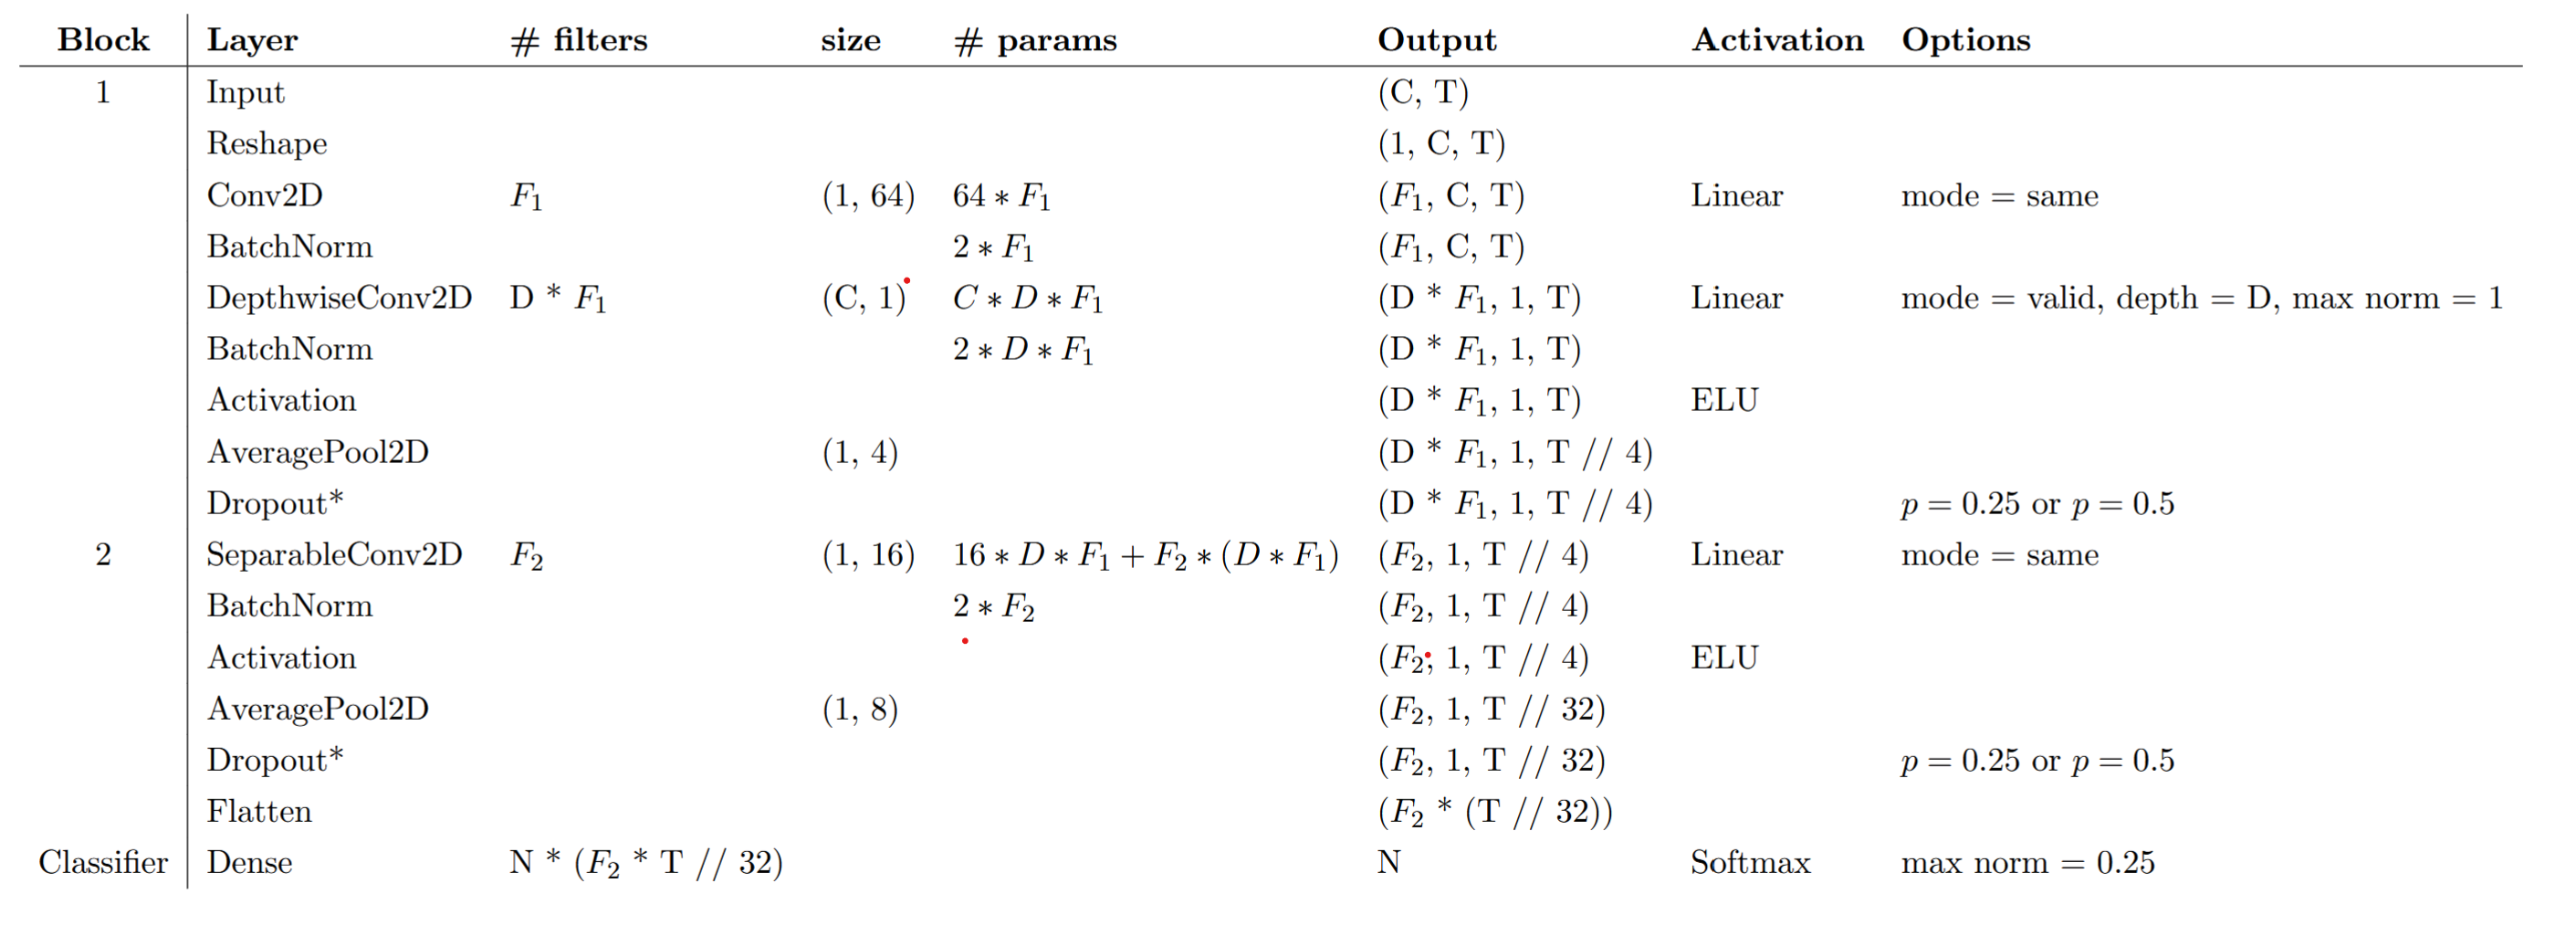
\includegraphics[scale=0.45]{gfx/MThes_EEGNetArchitectureDetailList.png} 
    \caption{Detailed list of the layers used in the EEGNet (taken from \cite{lawhern-2018})} % update image description?
    \label{app:EEGNetDetail}
\end{figure}

%\addcontentsline{toc}{chapter}{\listtablename}
%\listoftables
%\cleardoublepage

\pagestyle{empty}
% !TEX root = ../thesis-example.tex
%
%************************************************
% Declaration
%************************************************
\pdfbookmark[0]{Declaration}{Declaration}
\chapter*{Selbstständigkeitserklärung}
\label{sec:declaration}
\thispagestyle{empty}

Hiermit versichere ich, {\thesisName}, dass ich die von mir vorgelegte Arbeit
\emph{\thesisTitle} selbstständig verfasst und keine anderen als die angegebenen
Quelle und Hilfsmittel verwendet habe.

\smallskip

\noindent\textit{\thesisUniversityCity, \thesisDate}

\smallskip

\begin{flushright}
	\begin{minipage}{5cm}
		\rule{\textwidth}{1pt}
		\centering\thesisName
	\end{minipage}
\end{flushright}

%*****************************************
%*****************************************

\clearpage
\newpage
\mbox{}

% **************************************************
% End of Document CONTENT
% **************************************************
\end{document}
